\begingroup %{
\newcommand{\C}{\mycal{C}}
\newcommand{\D}{\mycal{D}}
\newcommand{\E}{\mycal{E}}
\newcommand{\F}{\mycal{F}}
\newcommand{\I}{\mycal{I}}
\newcommand{\J}{\mycal{J}}
\newcommand{\M}{\mycal{M}}
\newcommand{\Q}{\mycal{Q}}
\newcommand{\T}{\mycal{T}}
\newcommand{\W}{\mycal{W}}
\newcommand{\Z}{\mycal{Z}}
\newcommand{\Pow}{\mycal{P}}
\newcommand{\End}{\myop{End}}
\newcommand{\Map}{\myop{Map}}
\newcommand{\Lin}{\mathcal{L}}
\newcommand{\Etaol}{\mathcal{H}}
\newcommand{\Aut}{\myop{Aut}}
\newcommand{\Mat}{\myop{Mat}}
\newcommand{\Etaom}{\myop{Hom}}
\newcommand{\Eta}{\mycal{H}}
%
\newcommand{\id}{\myop{id}}
\newcommand{\tran}{\mathbf{t}}
\newcommand{\dfn}{\,\myop{def}\,}
\newcommand{\xiff}[2][]{\xLongleftrightarrow[#1]{#2}}
\newcommand{\tr}{\myop{tr}}
%
\newcommand{\mvec}[2]{\begin{matrix}{#1}\\{#2}\end{matrix}}
\newcommand{\mvect}[2]{\begin{matrix}{#1}&{#2}\end{matrix}}
\newcommand{\pvec}[2]{\begin{pmatrix}{#1}\\{#2}\end{pmatrix}}
\newcommand{\pvect}[2]{\begin{pmatrix}{#1}&{#2}\end{pmatrix}}
\newcommand{\bvec}[2]{\begin{bmatrix}{#1}\\{#2}\end{bmatrix}}
\newcommand{\bvect}[2]{\begin{bmatrix}{#1}&{#2}\end{bmatrix}}
\newcommand{\ad}{\myop{ad}}
\newcommand{\Ad}{\myop{Ad}}
%
\newcommand{\smallxy}[1]{\vcenter{\xymatrix@R=4pt@C=4pt@M=1pt@W=1pt{#1}}}
\newcommand{\hen}{\ar@{-}}
\newcommand{\sbt}{\vcenter{\hbox{\tiny$\bullet$}}}
%
\newcommand{\what}{\widehat}
\newcommand{\rvec}[1]{\overrightarrow{#1}}
\newcommand{\lvec}[1]{\overleftarrow{#1}}
%
{\setlength\arraycolsep{2pt}
%
\section{指数写像}\label{s1:指数写像} %{
	与えられた$\plr{x|t}\in\fukuso_q[[t]]$に対して
	\begin{equation*}\begin{split}
		\plr{\partial_t}_q\plr{y|t} = \plr{x|t}\plr{y|t}
	\end{split}\end{equation*}
	となる$\plr{y|t}\in\fukuso_q[[t]]$を求めることを考える。
	$\plr{x|t}=kx$の場合は、$\plr{y|t}=\plr{kx}_q^*\text{const.}$となるが、
	$\plr{x|t}$が一般の関数の場合は、次のようになる。
	\begin{equation*}\begin{split}
		\plr{y|t} \propto \plr{\I_qx|t} \quad\text{where}\quad 
		\plr{\I_qx|t} := 1 + \int_0^t\plr{x|s}\plr{\I_qx|s}d_qs
	\end{split}\end{equation*}
	ここで定義した$\I_qx$は、$q=1$のときのみ、次の式が成り立つことから
	(ノート\ref{note:積分計算その一})、
	\begin{equation}\label{eq:繰り返し積分その一}\begin{split}
		\frac{1}{n!}\plr{\int_0^t\plr{x|s}ds}^n
		= \int_0^t\plr{x|t_1}\int_0^{t_1}\plr{x|t_2}\cdots
			\int_0^{t_{n-1}}\plr{x|t_{n}}dt_{n}\cdots dt_2 dt_1
	\end{split}\end{equation}
	次のように$\exp$で書くことができる。
	\begin{equation*}\begin{split}
		\plr{\I_1x|t} = \plr{\exp\bou\int_0^t\plr{x|s}ds}
	\end{split}\end{equation*}

	\begin{note}[積分計算その一]\label{note:積分計算その一} %{
		$\plr{x|t}\in\fukuso[[t]]$とする。
		\begin{equation*}\begin{split}
			\plr{x|t} := \sum_{n\in\sizen} x_nt^n \quad\text{where } 
			x_n\in\fukuso
		\end{split}\end{equation*}
		次の二つの積分は一見異なるように見えるが、
		\begin{equation*}\begin{split}
			\plr{\int_0^t\plr{x|u}du}^2 &= \sum_{m,n\in\sizen} 
				\frac{x_mx_nt^{m+n+1}}{(m+1)(n+1)} \\
			\int_0^t\plr{x|u}\int_0^u\plr{x|v}dudv &= \sum_{m,n\in\sizen} 
				\frac{x_mx_nt^{m+n+1}}{(m+n+1)(n+1)} \\
		\end{split}\end{equation*}
		二つ目の級数の和を対称化すると、次の式が得られる。
		\begin{equation*}\begin{split}
			&\int_0^t\plr{x|u}\int_0^u\plr{x|v}dudv \\
			&= \sum_{m,n\in\sizen} \frac{x_mx_nt^{m+n+1}}{(m+n+1)(n+1)} \\
			&= \frac{1}{2}\sum_{m,n\in\sizen} x_mx_nt^{m+n+1}
				\plr{\frac{1}{(m+n+1)(n+1)} + \frac{1}{(m+n+1)(m+1)}} \\
			&= \frac{1}{2}\sum_{m,n\in\sizen} 
				\frac{x_mx_nt^{m+n+1}}{(m+1)(n+1)} \\
			&= \frac{1}{2}\plr{\int_0^t\plr{x|u}du}^2
		\end{split}\end{equation*}
		同様にして\eqref{eq:繰り返し積分その一}を導き出す。
	\end{note} %note:積分計算その一}
%s1:指数写像}
\section{有理式体}\label{s1:有理式体} %{
	$R$を標数$0$の整域、$R[t]$を$R$上の多項式環、$R[t]_\times:=R[t]-\set{0}$
	とする。$R[t]\times R[t]_\times$に積を次のように定義すると、
	\begin{equation*}\begin{split}
		\plr{x_1\times x_2}\plr{y_1\times y_2} := x_1y_1\times x_2y_2
		\quad\text{for all } x_i\in R[t],\; y_i\in R[t]_\times
	\end{split}\end{equation*}
	$1\times1$を単位元とするモノイドとなる。
	$R[t]\times R[t]_\times$に関係$\sim$を次のように定義すると、
	\begin{equation*}\begin{split}
		x_1\times x_2\sim y_1\times y_2 \xiff{\dfn} 
		\text{there exists } z\in R[t] \text{ such that } x_1y_2z = x_2y_1z \\
		\quad\text{for all } x_i\in R[t],\; y_i\in R[t]_\times
	\end{split}\end{equation*}
	$\sim$は同値関係になり、同値類
	$\Q R[t]:=\plr{R[t]\times R[t]_\times}/\sim$が定義できる。
	$\Q R[t]$の元を割り算の記号を用いて$x/y$と書く。$\Q R[t]$は零元$0/1$
	を持ち、$0/1$以外は逆元を持つモノイドとなる。
	入射$\iota:R[t]\to\Q R[t]$を次のように定義すると、
	\begin{equation*}\begin{split}
		\iota x := x / 1 \quad\text{for all } x\in R[t]
	\end{split}\end{equation*}
	$\iota$は$1:1$のモノイド射となる。$\iota$が代数射になるように、
	$\Q R[t]$に加法を定義すると、次のようになる。
	\begin{equation*}\begin{split}
		\frac{x_1}{x_2} + \frac{y_1}{y_2}
		= \frac{x_1y_2 + x_2y_1}{x_2y_2}
		\quad\text{for all } x_i\in R[t],\; y_i\in R[t]_\times
	\end{split}\end{equation*}
	$\Q R[t]$を$R[t]$の有理式体という。$\Q R[t]$は$R$の局所化$\Q R$を
	含むので、通常は体上の多項式環の有理式体を考える。
%s1:有理式体}
\section{射影変換}\label{s1:射影変換} %{
	$\fukuso_\times:=\fukuso-\set{0}$、$\fukuso P_n$を$n$次元射影空間とする。

	$\fukuso P_1$の一次変換$T_i$を次のように定義すると、
	\begin{equation*}\begin{split}
		T_i\frac{x}{y} := \frac{a_ix + b_iy}{c_ix + d_iy}
		\quad\text{for all } i\in\sizen_+,\; x\in\fukuso,\; y\in\fukuso_\times
	\end{split}\end{equation*}
	一次変換の合成$T_2T_1$は次のようになる。
	\begin{equation*}\begin{split}
		T_2T_1\frac{x}{y} &= T_2\frac{a_1x + b_1y}{c_1x + d_1y}
		= \frac{a_2\plr{a_1x + b_1y} + b_2\plr{c_1x + d_1y}}
			{c_2\plr{a_1x + b_1y} + d_2\plr{c_1x + d_1y}} \\
		&= \frac{\pvect{a_2}{b_2}\pvec{a_1}{c_1}x
			+ \pvect{a_2}{b_2}\pvec{b_1}{d_1}y}{\pvect{c_2}{d_2}\pvec{a_1}{c_1}x
			+ \pvect{c_2}{d_2}\pvec{b_1}{d_1}y}
	\end{split}\end{equation*}
	したがって、次のようにカギ括弧の行列で一次変換を表すと、
	\begin{equation*}\begin{split}
		\begin{bmatrix}
			a & b \\ c & d
		\end{bmatrix}\frac{x}{y} := \frac{ax + by}{cx + dy}
	\end{split}\end{equation*}
	一次変換の合成は通常の行列の積で書くことができる。
	\begin{equation*}\begin{split}
		\begin{bmatrix}
			a_2 & b_2 \\ c_2 & d_2
		\end{bmatrix}\begin{bmatrix}
			a_1 & b_1 \\ c_1 & d_1
		\end{bmatrix} = \begin{bmatrix}
			a_2a_1 + b_2c_1 & a_2b_1 + b_2d_1 \\ c_2a_1 + d_2c_1 
			& c_2b_1 + d_2d_1
		\end{bmatrix}
	\end{split}\end{equation*}

	写像$\iota:\fukuso\times\fukuso_\times\to\fukuso^2$と
	写像$\pi:\iota\plr{\fukuso\times\fukuso_\times}\to\fukuso P_1$を
	次のように定義すると、
	\begin{equation*}\begin{split}
		\iota(x, y) := \pvec{x}{y} ,\quad\pi\pvec{x}{y} := \frac{x}{y} 
		\quad\text{for all } x\in\fukuso,\; y\in\fukuso_\times
	\end{split}\end{equation*}
	次の可換図が成り立つ。
	\begin{equation*}\xymatrix@C=4em{
		x\times y \ar@{|->}[d]^\iota \ar@{|->}[r]^T
			& \plr{ax + by}\times\plr{cx + dy} \ar@{|->}[d]^\iota \\
		\,\pvec{x}{y} \ar@{|->}[d]^\pi \ar@{|->}[r]^{\begin{pmatrix}
			a & b \\ c & d
		\end{pmatrix}} & \,\pvec{ax + by}{cx + dy} \ar@{|->}[d]^\pi \\
		\cfrac{x}{y} \ar@{|->}[r]^{\begin{bmatrix}
			a & b \\ c & d
		\end{bmatrix}}& \cfrac{ax + by}{cx + dy} \\
	}\end{equation*}
%s1:射影変換}
\section{代数式と差分式の関係}\label{s1:代数式と差分式の関係} %{
	$R$を標数$0$の整域(ノート\ref{note:整域の標数})、$R_q$を多項式$R[q]$に
	よる有理式体とする。

	線形射$\I_q^t:R[x]\to R[[t]]$を次のように再帰的に定義する。
	\begin{equation}\label{eq:多項式から形式級数への線形射}\begin{split}
		\I_q^t f = 1 + \int_0^t\plr{f\bou\I_q^sf}d_qs
		\quad\text{for all } f\in R[x]
	\end{split}\end{equation}
	ここでは、$\I_q^t$が定義できるかどうかは置いておき、この代数式で
	定義できるものとする\footnote{
		$R$が標数$0$の整域でない場合は、再帰式
		\eqref{eq:多項式から形式級数への線形射}の解が複数あり得る。
		また、$R$が標数$0$の整域という条件だけで、解が唯一つ定まるかどうかも
		わからない。
	}。すると、$\I_q^tf$は次の微分方程式を満たす。
	\begin{equation*}\begin{split}
		\plr{\partial_t}_q\plr{I_q^tf} = \plr{f\bou\I_q^tf},\quad \I_q^0f = 1
	\end{split}\end{equation*}

	線形射$\I_q^t$にワンクッション挟んで、
	$R[x]\to R\D(\xi)\to R[[t]]$という線形射に分解する。線形射
	$\omega:R[x]\to R\D\braket{\xi,\bar{\xi}}$を次のように再帰的に定義する。
	\begin{equation*}\begin{split}
		\omega f = 1 + \xi\plr{f\bou\omega f}\bar{\xi}
		\quad\text{for all } f\in R[x]
	\end{split}\end{equation*}
	$\omega f$の各項は$\xi$と$\bar{\xi}$のバランスがとれているので、
	$\xi$と$\bar{\xi}$で生成されるDyck言語$\D(\xi)$の和になっている。
	したがって、$\omega:R[x]\to R\D(\xi)$となる。
	線形射$\iota_q^t:R\D(\xi)\to R_q[[t]]$を次のように再帰的に定義する。
	\begin{equation*}\begin{split}
		\iota_q^t1 &:= 1 \\
		\iota_q^t\plr{\xi w_1\bar{\xi}w_2} & := \int_0^t
		\plr{\iota_q^sw_1}\plr{\iota_q^sw_2}d_qs 
		\quad\text{for all } w_1,w_2\in \D(\xi)
	\end{split}\end{equation*}
	すると、次の式が成り立ち、
	\begin{equation*}\begin{split}
		\iota_q^t\omega f = 1 + \int_0^t \plr{f\bou\iota_q^s\omega f} d_qs
		\quad\text{for all } f\in R[x]
	\end{split}\end{equation*}
	$\iota_q^t\omega=\I_q^t$となる。

	多項式$\plr{f\bou x}\in R[x]$に対して明示的に書くと次のようになっている。
	\begin{equation*}\begin{array}{rclclclclcl}
		\plr{f\bou x} &:=& && a_0 &+& a_1x &+& a_2x^2 &+& \cdots \\
		\omega f &=& 1 &+& a_0\xi\bar{\xi} &+& a_1\xi\plr{\omega f}\bar{\xi} 
			&+& a_2\xi\plr{\omega f}^2\bar{\xi} &+& \cdots \\
		\iota_q^t\omega f &= &1 &+& a_0t 
			&+& a_1\int_0^t\plr{\iota_q^s\omega f}d_qs
			&+& a_2\int_0^t\plr{\iota_q^s\omega f}^2d_qs &+& \cdots \\
	\end{array}\end{equation*}
	$\omega f$をBrzozowski代数を使って書くと次のようになる。
	\begin{equation*}\begin{split}
		\omega f = \pvec{1}{0}^\tran\braket{T^*}\pvec{0}{1}
		,\quad T = \begin{pmatrix}
			\xi h_{11} & 1 + a_0\xi\bar{\xi} \\ h_{21} & h_{22}\bar{\xi}
		\end{pmatrix} \\
	\end{split}\end{equation*}
	ここで、$h_{ij}\in R\Eta_*$は次のように定義する。
	\begin{equation*}\begin{split}
		h_{11} := \sum_{n=1}^{\deg f} a_n\eta_{n1},\quad
		h_{21} := \sum_{n=2}^{\deg f} \sum_{k=1}^{n-1} 
			\eta_{nk}^\flat\eta_{n(k+1)},\quad
		h_{22} := \sum_{n=1}^{\deg f} \eta_{nn}^\flat
	\end{split}\end{equation*}
	行列$T$のBrzozowski代数の階数は$\plr{\deg f}\plr{\deg f+1}/2$となる。

	\begin{note}[整域の標数]\label{note:整域の標数} %{
		$R$を整域とする。$n\in\sizen$を$n1=0$となる最小の自然数とする。
		ある$p,q\in\sizen$で$n=pq$と書けたとすると、$n1=\plr{p1}\plr{q1}=0$
		となる。$R$は整域だから、$p1=0$または$q1=0$となるが、それは$n$の定義に
		反する。したがって、$n$は$0$または素数でなくてはならない。
		つまり、整域の標数は$0$または素数に限られる。
	\end{note} %note:整域の標数}
%s1:代数式と差分式の関係}
\section{Riccati方程式}\label{s1:Riccati方程式} %{
	定数を係数とするRiccati方程式を考える。

	$a,b,c\in\fukuso$として次のq-微分方程式を考える。
	\begin{equation}\label{eq:定係数Riccati}\begin{split}
		\plr{\partial_t}_q\plr{x|t} = a + b_1\plr{x|t} 
			+ b_2\plr{x|qt} + c\plr{x|t}\plr{x|qt}
	\end{split}\end{equation}
	\Midline{q-微分をバラすと次の式が得られる。}次の式は間違っている。
	\begin{equation*}\begin{split}
		\plr{x|t} = \ggplr{1 - \plr{1 - q}tT}\begin{pmatrix}
			\plr{x|qt} \\\hline 1
		\end{pmatrix} \quad\text{where } T := \begin{pmatrix}
			- b_2 & - a \\ c & b_1
		\end{pmatrix}
	\end{split}\end{equation*}
	ここで、右辺は射影変換を表す。$|q|<1$ならば、\eqref{eq:定係数Riccati}
	の解は次の積表示を持つ。
	\begin{equation*}\begin{split}
		\plr{x|t} = \prod_{n\in\sizen}\ggplr{1 - (1-q)q^ntT} \begin{pmatrix}
			\plr{x|0} \\\hline 1
		\end{pmatrix} \quad\text{when } |q| < 1
	\end{split}\end{equation*}
	この式の右辺はq-Kleeneスターの逆数(節\eqref{s2:q-Kleeneスター})に
	なっているので、次のように書くことができる。
	\begin{equation*}\begin{split}
		\plr{x|t} = \plr{tT}_q^{-*} \begin{pmatrix}
			\plr{x|0} \\\hline 1
		\end{pmatrix}
		= \sum_{n\in\sizen} q^{\binom{n}{2}}\frac{\plr{-tT}^n}{[n]_q!}
		\begin{pmatrix}
			\plr{x|0} \\\hline 1
		\end{pmatrix} \\\quad\text{when } |q| < 1 \text{ or } q = 1
	\end{split}\end{equation*}
	この式は$q=1$でも定義できることに注意する\footnote{
		$|q|=1$では$[n]_q!$が$0$になり得るので、$|q|=1$では定義できない。
		$q=1$の時のみ$[n]_q!$が$0$にならない。
	}。

\subsubsection{双線形化による解法}\label{s3:双線形化による解法} %{
	教科書\cite{hirota:2003}にならって定係数Riccati\eqref{eq:定係数Riccati}
	を解いてみる。次の変数変換をして、
	\begin{equation*}\begin{split}
		\plr{x|t} := \frac{\plr{f|t}}{\plr{g|t}}
	\end{split}\end{equation*}
	次の微分を使うと\footnote{
		次のように微分をとることもできるが、
		\begin{equation*}\begin{split}
			\plr{\partial_t}_q\frac{\plr{f|t}}{\plr{g|t}}
			= \plr{\partial_t}_q\plr{\plr{f|t}\frac{1}{\plr{g|t}}}
			= \frac{\plr{f|D_q|t}\plr{g|qt} 
				- \plr{f|t}\plr{g|D_q|t}}{\plr{g|qt}\plr{g|t}}
		\end{split}\end{equation*}
		この場合、ゲージ対称性が明白でなくなる、もしくは、ゲージ対称性がない。
	}、
	\begin{equation*}\begin{split}
		\plr{\partial_t}_q\frac{\plr{f|t}}{\plr{g|t}}
		= \plr{\partial_t}_q\plr{\frac{1}{\plr{g|t}}\plr{f|t}}
		= \frac{\plr{f|D_q|t}\plr{g|t} 
			- \plr{t|f}\plr{g|D_q|t}}{\plr{g|qt}\plr{g|t}}
	\end{split}\end{equation*}
	次の双線形な微分方程式が得られる。
	\begin{equation}\label{eq:定係数Riccatiの双線形}\begin{split}
		&\plr{f|D_q|t}\plr{g|t} - \plr{f|t}\plr{g|D_q|t} \\
		&= a\plr{g|t}\plr{g|qt} + b_1\plr{f|t}\plr{g|qt}
			+ b_2\plr{g|t}\plr{f|qt} + c\plr{f|t}\plr{f|qt}
	\end{split}\end{equation}
	任意の正則関数$\plr{h|t}$による次のゲージ変換で、
	\begin{equation*}\begin{split}
		\plr{f|t} \mapsto \plr{h|t}\plr{f|t}
		,\quad \plr{g|t} \mapsto \plr{h|t}\plr{g|t}
		\quad\text{for all } \plr{h|t}
	\end{split}\end{equation*}
	\eqref{eq:定係数Riccatiの双線形}は不変になっている。
	\begin{equation*}\begin{split}
		\text{l.h.s.} \mapsto \plr{h|t}\plr{h|qt}\plr{\text{l.h.s.}}
		,\quad \text{r.h.s.} \mapsto \plr{h|t}\plr{h|qt} \plr{\text{r.h.s.}}
	\end{split}\end{equation*}
	\eqref{eq:定係数Riccatiの双線形}を次のように書き直して、
	\begin{equation*}\begin{split}
		\frac{\plr{f|D_q|t} - a\plr{g|qt} - b_2\plr{f|qt}}{\plr{f|t}}
		= \frac{\plr{g|D_q|t}+ b_1\plr{g|qt} + c\plr{f|qt}} {\plr{g|t}}
	\end{split}\end{equation*}
	両辺を$\plr{\alpha|t}$とおくと、次の連立微分方程式が得られる。
	\begin{equation*}\begin{split}
		\plr{f|D_q|t} - a\plr{g|qt} - b_2\plr{f|qt} 
		&= \plr{\alpha|t}\plr{f|t} \\
		\plr{g|D_q|t} + b_1\plr{g|qt} + c\plr{f|qt} &= \plr{\alpha|t}\plr{g|t}
	\end{split}\end{equation*}
	この式に対して次のゲージ変換を使うと、
	\begin{equation*}\begin{split}
		\plr{f|t}\mapsto \plr{f|t}\int_0^t\plr{\alpha|s}d_qs
		,\quad \plr{t|t}\mapsto \plr{g|t}\int_0^t\plr{\alpha|s}d_qs
	\end{split}\end{equation*}
	ゲージ場$\alpha$を消去した次の式が得られる。
	\begin{equation*}\begin{split}
		\plr{f|D_q|t} - a\plr{g|qt} - b_2\plr{f|qt} &= 0 \\
		\plr{g|D_q|t} + b_1\plr{g|qt} + c\plr{f|qt} &= 0
	\end{split}\end{equation*}
%s3:双線形化による解法}
%s1:Riccati方程式}
\section{代数的Chomsky-Schutzenbergerの定理}\label{s1:代数的Chomsky-Schutzenbergerの定理} %{
	Wikipeidaに代数的Chomsky-Schutzenbergerの定理の項目\footnote{
		英語のWikipediaで次の文字列で検索すればよい。
		\begin{itemize}\setlength{\itemsep}{-1mm} %{
			\item Chomsky-Schutzenberger
		\end{itemize} %}
	}があったので記録しておく。

	$\sizen[[x]]$を自然数を係数とする形式級数全体のつくる集合、
	$\bun(x):=\bun[x,x^{-1}]$を有理数を係数とする$x$と$x^{-1}$を変数とする
	多項式全体のつくる集合とする。

	$f\in\sizen[[x]]$が次の性質を満たす時、$f$を$\bun(x)$上で代数的という。
	\begin{itemize}\setlength{\itemsep}{-1mm} %{
		\item ある有限個の$p_0,\dots,p_n\in\bun(x)$が存在して、
		\begin{equation*}\begin{split}
			p_0 + p_1\cdot f +\cdots+ p_n\cdot f^n = 0
		\end{split}\end{equation*}
		となる。ここで、積$\cdot$は次のように定義する。
		\begin{equation*}\begin{split}
			\plr{\phi\cdot\psi|x} := \plr{\phi|x}\plr{\psi|x}
		\end{split}\end{equation*}
	\end{itemize} %}

	\begin{proposition}[代数的Chomsky-Schutzenberの定理]\label{prop:代数的Chomsky-Schutzenberの定理} %{
		$A$を有限集合、$L\subseteq A^*$を曖昧さのない文脈自由文法、
		$L_n:=\set{w\in L\bou |w|=n}$とする。
		このとき、$\sum_{n\in\sizen}|L_n|t^n$は$\bun(t)$上で代数的となる。
	\end{proposition} %prop:代数的Chomsky-Schutzenberの定理}

	$A$を文字集合、$f\in\sizen\braket{A,x}$として、
	文法$x=\plr{f|x}$に曖昧さがなければ、ある言語$L\subseteq A^*$があって、
	$x=\sum_{w\in L}w$と摂動展開が書ける。
	したがって、モノイド射$\chi_t:A^*\to\set{t}^*$を$\chi_tw=t^{|w|}$と定義i
	して、それを線形に拡張すると、$\chi_tx=\sum_{n\in\sizen}|L_n|t^n$となる。
	$A$が有限集合だから、任意の$n\in\sizen$で$L_n\le|A^n|=|A|^n$となり、
	少なくとも$|t|<|A|^{-1}$では$\chi_tx$は収束する。
	そして、$\chi_t$を文法に作用させると、$\chi_tx=\chi_t\plr{f|x}$という
	形式級数に対する代数式が得られる。
	
	例を使って考えてみよう。
	文字集合$A:=\set{p,m,l,r,v}$から生成される次の文法を考える。
	\begin{equation*}\begin{split}
		X &= Y + YpX + YmX,\quad Y = v^* + lXr 
	\end{split}\end{equation*}
	任意の$\alpha\in A$に対して$\chi_t\alpha=t$だから、文法に$\chi_t$を作用
	させると、次のようになる。
	\begin{equation*}\begin{split}
		\left\{\begin{split}
			X_t &= Y_t + 2tY_tX_t \\
			Y_t &= t^* + t^2X_t
		\end{split}\right. \iff \left\{\begin{split}
			X_t &= \plr{t^* + t^2X_t}\plr{1 + 2tX_t} \\
			Y_t\plr{1 - 2tY_t} &= t^*\plr{1 - 2tY_t} + t^2Y_t
		\end{split}\right.
	\end{split}\end{equation*}
	Kleeneスターを展開しても次のようになり、
	\begin{equation*}\begin{split}
		\plr{1 - t}X_t &= \plr{1 + \plr{1 - t}t^2X_t}\plr{1 + 2tX_t} \\
		\plr{1 - 1}Y_t\plr{1 - 2tY_t} &= \plr{1 - 2tY_t} + t^2Y_t
	\end{split}\end{equation*}
	この文法は$\sizen[t]$上で代数的になる。
	普通に考えると、曖昧さがない文脈自由文法は$\sizen[t]$上で代数的になりそう
	なものだが、何か見落としているのだろう。

	曖昧さがある文脈自由文法の場合、文法の摂動解$x$の各項に組合せの数が係数が
	掛かり、$\chi_tx$の収束半径が有限になるかどうかが簡単に判断できなくなる。
	しかし、曖昧さは新たな不定元を追加することで回避できることがある。
	例えば、次のような変形である。
	\begin{equation*}\begin{split}
		x = a + xbx \mapsto x = a + xbxc
	\end{split}\end{equation*}
	したがって、すべての曖昧な文法に対して、新たな不定元を追加することで
	曖昧さが回避できるならば、代数的Chomsky-Schutzenberの定理から
	曖昧さの制限を取り除くことができる。

	代数的Chomsky-Schutzenberの定理は自由モノイドに対する命題だが、Kontsevich
	\cite{2011arXiv1109.2469K}によって自由群に対して同様の命題が証明されて
	いる。\cite{2011arXiv1109.2469K}ではより大きな目標の一貫として自由群に
	対する代数的Chomsky-Schutzenberの定理が証明されているようだが、
	Reutenauer達\cite{Reutenauer:2012}が、代数的Chomsky-Schutzenber
	の定理の部分だけを抜き出して解説している。
%s1:代数的Chomsky-Schutzenbergerの定理}
\section{環の中心}\label{s1:環の中心} %{
	$V$を環、$C$を$V$の中心とする。$C$は$0$と$1$を含むので、空ではない。
	また、$x,y\in C$なら、任意の$v\in V$に対して次のことが成り立つので、
	\begin{itemize}\setlength{\itemsep}{-1mm} %{
		\item $(x+y)r=r(x+y)$
		\item $xyr=rxy$
	\end{itemize} %}
	$C$は$V$の部分環となる。
%s1:環の中心}
\section{既約と分解可能}\label{s1:既約と分解可能} %{
	$S$を環、$V$を$S$上の加群とする。部分空間$W\subset V$が$SW\subseteq W$と
	なるとき、$W$を不変な部分空間という。
	不変な部分空間が$\set{0}$と$V$自身に限られるとき、$V$を既約な加群という。
	また、任意の不変な部分空間$W\subseteq V$に対して$V=W\oplus W'$と直和分解
	できるとき、$V$を分解可能または完全可約な加群という。
%s1:既約と分解可能}
\section{Brzozowski代数}\label{s1:Brzozowski代数} %{
	$R$を可換環、$A$を空でない有限集合とする。
	$A$から生成される$R$上のBrzozowski代数\footnote{
		q-Heisenberg代数の$q=0$としたものをBrzozowski代数と書いている。
	}を$R\Eta(A)$と書く。
	\begin{equation*}\begin{split}
		R\Eta(A) := \frac{R\braket{A,A^\flat}}
			{ab^\flat = \jump{a=b} \text{ for all }a,b\in A} 
	\end{split}\end{equation*}
	$R\Eta(A)$の基底を次のように書くことにする。
	\begin{itemize}\setlength{\itemsep}{-1mm} %{
		\item $A$の元を消滅演算子
		\item $A^\flat$の元を生成演算子
	\end{itemize} %}
	また、文字集合を明記する必要がない場合は、文字集合の大きさだけを明記
	して$R\Eta_n$と書き、文字集合について次の便宜を用いることにする。
	\begin{equation*}\begin{split}
		R\Eta_n := R\Eta(H_n) \quad\text{where } H_n := \set{\eta_1,\dots,e_n}
	\end{split}\end{equation*}
	\underline{逆順の}代数射$-^\flat:R\Eta(A)\to R\Eta(A)$を次のように定義する。
	\begin{equation*}\begin{split}
		(a)^\flat = a^\flat,\quad (a^\flat)^\flat = a
		\quad\text{for all } a\in A
	\end{split}\end{equation*}
	そして、$R\Eta_n$の場合は特別に次の約束を使う。
	\begin{equation*}\begin{split}
		\eta_i^\flat = \eta_{-i} \quad\text{for all } i\in1..n
	\end{split}\end{equation*}

\subsubsection{数演算子}\label{s3:数演算子} %{
	$\mu_n\in R\Eta(A)$を次のように定義する。
	\begin{equation*}\begin{split}
		\mu_n := \sum_{a\in A} (a^\flat)^na^n \quad\text{for all } n\in\sizen
	\end{split}\end{equation*}
	集合$M\subset R\Eta(A)$を$M:=\set{\mu_n\bou n\in\sizen}$と定義すると、
	次の式から、
	\begin{equation*}\begin{split}
		\mu_m\mu_n = \mu_{\max(m,n)} \quad\text{for all } m,n\in\sizen
	\end{split}\end{equation*}
	$M$はモノイドとなり、モノイド同型$M\simeq(\sizen,\max,0)$が成り立つ。
	また、$M$の元はすべてべき等$\mu_n^2=\mu_n$になる。
	特に、$\what{N}_0:=\mu_1$と定義し、$\what{N}_0$を数演算子ということに
	する。
%s3:数演算子}

\subsubsection{Fock空間}\label{s3:Fock空間} %{
	係数環$R$が複素数の場合は、$\what{N}_0$はべき等なので、固有値は$0$と$1$
	だけになることが言える。$\what{N}_0$の固有値を拠り所にして表現を考える
	ために、係数環を複素数に限定する。

	$\fukuso\Eta(A)$の表現空間は、$\what{N}_0$の固有値によって次の三種類
	に分類される。
	\begin{enumerate}\setlength{\itemsep}{-1mm} %{
		\item $\what{N}_0$の固有値を$0$だけ持つ。
		\item $\what{N}_0$の固有値を$1$だけ持つ。
		\item $\what{N}_0$の固有値を$0$と$1$の両方持つ。
	\end{enumerate} %}
	ここでは、三番目の$\what{N}_0$の固有値を$0$と$1$の両方持つ表現空間を
	考える。

	$V$を$\fukuso\Eta(A)$の表現空間とし、$V_\lambda$を$\what{N}_0$の固有値
	$\lambda$を持つ$V$の部分空間とすると、$V=V_0\oplus V_1$と直和分解される。
	そして、$V_0$と$V_1$は空でないとする。任意の$a\in A$に対して次の性質が
	成り立つ。
	\begin{enumerate}\setlength{\itemsep}{-1mm} %{
		\item $\ker a^\flat=\set{0}$となる。\\
		ある$v\in V$に対して$a^\flat v=0$ならば、左から$a$を作用させると、
		$v=0$となる。
		%
		\item $\ker a=V_0$となる。\\
		任意の$v\in V_0$に対して$\what{N}_0v=0$となるが、左から$a$を作用させる
		と、$av=0$となる。したがって、$V_0\subseteq \ker a$となる。
		一方、$\what{N}_0$の定義より、$\ker a\subseteq V_0$となるから、
		$\ker a=V_0$となることがわかる。
		%
		\item $a^\flat V\subseteq V_1$となる。\\
		任意の$v\in V$に対して$\what{N}_0a^\flat v=a^\flat v$となる。
		%
		\item 任意の$v\neq0\in V_0$と$n\in\sizen$に対して
		$\Set{(a^\flat)^nv\bou n\in\sizen}$は線形独立となる
		(ノート\ref{note:自然数による基底系})。
	\end{enumerate} %}
	そして、次の性質が成り立つ。
	\begin{enumerate}\setlength{\itemsep}{-1mm} %{
		\item 任意の$v\neq0\in V_0$に対して集合$(A^\flat)^*v\subset V$を
		$(A^\flat)^*v:=\Set{w^\flat v\bou w\in A^*}$と定義すると、
		$(A^\flat)^*v$の元は互いに線形独立となる
		(ノート\ref{note:単語による基底系})。
		したがって、任意の$v\neq0\in V_0$に対してモノイド環$\fukuso\braket{A}$
		との線形同型$\fukuso(A^\flat)^*v\simeq\fukuso\braket{A}$が成り立つ。
		%
		\item $u,v\in V_0$が互いに線形独立であれば、直和分解
		$\fukuso(A^\flat)^*u\cup\fukuso(A^\flat)^*v
		=\fukuso(A^\flat)^*u\oplus\fukuso(A^\flat)^*v$が成り立つ
		(ノート\ref{note:真空の独立性})。
	\end{enumerate} %}
	したがって、次の部分空間の関係が成り立つ。
	\begin{equation*}\begin{split}
		\plr{\fukuso\braket{A}}^{\oplus\plr{\dim\ker\what{N}_0}} \subseteq V
		\quad\text{as vector space}
	\end{split}\end{equation*}
	また、$\what{N}_0$の固有値が$0$と$1$の両方を持つような$\fukuso\Eta(A)$
	の$\fukuso\braket{A}$への表現は既約表現となる
	(ノート\ref{note:Fock表現の既約性})。
	以上を定義と命題の形でまとめておく。

	\begin{definition}[Fock表現]\label{def:Fock表現} %{
		$R$を可換環、$A$を空でない有限集合、$R\Eta(A)$を$R$上のBrzozowski代数
		とする。$R\Eta(A)$の自由モノイド環$R\braket{A}$への次の表現をFock表現
		ということにする。
		\begin{alignat*}{2}
			a\ket{1} &= 0 &\quad&\text{for all } a\in A \\
			a\ket{bw} &= \jump{a=b}\ket{w} 
				&\quad&\text{for all } a,b\in A,\; w\in A^* \\
			a^\flat\ket{w} &= \ket{aw} 
				&\quad&\text{for all } a\in A,\; w\in A^*
		\end{alignat*}
		ここで、$\fukuso\Eta(A)$の基底系と$\fukuso\braket{A}$の基底系を区別
		するために、$\fukuso\braket{A}$の基底系をブラケット記法を使って書いた。
	\end{definition} %def:Fock表現}

	\begin{proposition}[Fock表現の既約性]\label{prop:Fock表現の既約性} %{
		複素数上のBrzozowski代数のFock表現は既約表現である。
	\end{proposition} %prop:Fock表現の既約性}

	\begin{proposition}[数演算子による表現の分類]\label{prop:数演算子による表現の分類} %{
		$A$を空でない有限集合、$\fukuso\Eta(A)$を複素数上のBrzozowski代数
		とする。$\fukuso\Eta(A)$の表現$(\rho,V)$が、$\what{N}_0$の固有値
		$0$と$1$の両方を持てば、次の部分空間の関係が成り立つ。
		\begin{equation*}\begin{split}
			\plr{\fukuso\braket{A}}^{\oplus\plr{\dim\ker\what{N}_0}} \subseteq V
			\quad\text{as vector space}
		\end{split}\end{equation*}
	\end{proposition} %prop:数演算子による表現の分類}

	\begin{note}[自然数による基底系]\label{note:自然数による基底系} %{
		任意の$v\neq0\in V_0$と$n\in\sizen$に対して
		$\Set{(a^\flat)^iv\bou i\in0..n}$は線形独立となる。
		\begin{proof} %{
			$n$に関する帰納法を使う。$n=0$の時は明らかで、ある$n\in\sizen$で
			命題が成り立つとすると、任意の$c_1,\dots,c_{n+1}\in\fukuso$に対して
			次の式が成り立つ。
			\begin{alignat*}{2}
				& c_1(a^\flat)v +\cdots+ c_{n+1}(a^\flat)^{n+1}v = 0 \\
				\iff & a^\flat\plr{c_1v +\cdots+ c_{n+1}(a^\flat)^nv} = 0 \\
				\implies & c_1v +\cdots+ c_{n+1}(a^\flat)^nv = 0 
					&\quad& \because\quad \ker a^\flat = \set{0} \\
				\implies & c_1v = 0 \text{ and } 
					c_2v +\cdots+ c_{n+1}(a^\flat)^nv = 0
					&\quad& \because\quad V_0\cup V_1 = \set{0} \\
				\implies & c_1 = c_2 =\cdots= c_{n+1} = 0
					&\quad& \text{by assumptions}
			\end{alignat*}
		\end{proof} %}
	\end{note} %note:自然数による基底系}

	\begin{note}[単語による基底系]\label{note:単語による基底系} %{
		任意の$v\neq0\in V_0$、$n\in\sizen$に対して集合
		$(A^\flat)^n v\subseteq V$を次のように定義し、
		\begin{equation*}\begin{split}
			(A^\flat)^n v := \Set{w^\flat v\bou w\in A^n}
		\end{split}\end{equation*}
		$(A^\flat)^{\le n} v:=\cup_{r=0}^n(A^\flat)^r v$とする。
		任意の$n\in\sizen$に対して$(A^\flat)^{\le n} v$の元は互いに線形独立
		になる。
		\begin{proof} %{
			$(A^\flat)^{\le n} v$の$n$についての帰納法で証明する。
			$n=0$のときは$(A^\flat)^{\le 0} v=\fukuso v$だから、命題が成り立つ
			ことがわかる。ある$n\in\sizen$で命題が成り立つと仮定する。
			写像$c:A^{n+1}\to\fukuso$が次の式を満たすとすると、
			\begin{equation*}\begin{split}
				\sum_{w\in A^{n+1}} \plr{c|w}w^\flat v = 0
			\end{split}\end{equation*}
			任意の$a\in A$で次の式が成り立つ。
			\begin{alignat*}{2}
				a\sum_{w\in A^n} \plr{c|w} w^\flat v = 0
				\implies & \sum_{w\in A^n} \plr{c|wa} w^\flat v = 0 \\
				\implies & \plr{c|wa} = 0 \quad\text{for all } w\in A^n
					&\quad& \text{by assumption}
			\end{alignat*}
			任意の$k\in\sizen$で$A^{k+1}=\cup_{a\in A}A^ka$が成り立つから、
			$c=0$となることがわかる。したがって、$n+1$でも命題が成り立つことが
			わかる。
		\end{proof} %}
	\end{note} %note:単語による基底系}

	\begin{note}[真空の独立性]\label{note:真空の独立性} %{
		ある$u,v\in V_0$、$w\in A^*$と写像$c:A^*\to\fukuso$が次の式を
		満たすとすると、
		\begin{equation*}\begin{split}
			w^\flat v = \sum_{x\in A^*} (c|x)x^\flat u
		\end{split}\end{equation*}
		次の式から、
		\begin{equation*}\begin{split}
			w^\flat v = \sum_{x\in A^*} (c|x)x^\flat u
			\implies v = \sum_{x\in A^*} (c|xw)x^\flat u \\
			\implies (c|w) u = v \quad\text{and}\quad
			(c|xw) = 0 \quad\text{for all } w\in A^+
		\end{split}\end{equation*}
		$u$と$v$は互いに線形従属となる。したがって、$u,v\in V_0$が互いに
		線形独立であれば、$(A^\flat)^*u$と$(A^\flat)^*v$は互いに線形独立
		となり、$(A^\flat)^*u\cup(A^\flat)^*v=(A^\flat)^*u\oplus(A^\flat)^*v$
		となる。
	\end{note} %note:真空の独立性}

	\begin{note}[Fock表現の既約性]\label{note:Fock表現の既約性} %{
		部分空間$V\subseteq\fukuso\braket{A}$を$\fukuso\Eta(A)$-不変な部分空間
		とする。
		\begin{itemize}\setlength{\itemsep}{-1mm} %{
			\item $V$が$\what{N}_0$の固有値$0$を持てば、$V=\set{0}$または
			$\fukuso\ket{1}\subseteq V$となる。$\fukuso\ket{1}$を含む
			$\fukuso\Eta(A)$-不変な部分空間は$\fukuso\braket{A}$だけだから、$V$は
			$\set{0}$または$\fukuso\braket{A}$自身となる。
			%
			\item $V$が$\what{N}_0$の固有値$1$のみを持てば、$V\subseteq\fukuso A^+$
			となる。ここで、
			$\fukuso A^+:=\myop{span}_\fukuso\Set{\ket{w}\bou w\in A^+}$とする。
			しかし、任意の$w\in A^+$に対して$w\ket{w}=\ket{1}$となるから、
			$\fukuso A^+$は$\fukuso\Eta(A)$-不変な部分空間ではなく、
			その部分空間もまた$\fukuso\Eta(A)$-不変な部分空間でない。したがって、
			$\what{N}_0$の固有値$1$だけを持つ$\fukuso\Eta(A)$-不変な
			$\fukuso\braket{A}$の部分空間は存在しない。
		\end{itemize} %}
		したがって、Fock表現は既約表現となる。
	\end{note} %note:Fock表現の既約性}

	\begin{note}[係数に対する制限]\label{note:係数に対する制限} %{
		係数に対する制限を弱めるためには、可換環$R$と$R$上の加群$V$が
		次の条件をクリアする必要がある。
		\begin{enumerate}\setlength{\itemsep}{-1mm} %{
			\item $V$でべき等作用素$T^2=T$の固有値が$0$と$1$だけになること。
			\item $V$が固有ベクトル空間で直和分解できること。
			\item 任意の$r\neq0\in R$と$v\neq0\in V$に対して$rv\neq0$
			となること。
		\end{enumerate} %}
		これらの条件は、$R$が整域で$V$が自由加群$R^D$であればクリアできると
		思う。
	\end{note} %note:係数に対する制限}

	\begin{todo}[この後の展開]\label{todo:この後の展開} %{
		この後の予定
		\begin{itemize}\setlength{\itemsep}{-1mm} %{
			\item Fock空間の内積を定義して、自由モノイドの積とその共役の作用版が
			Brzozowski代数となることを示す。
			\item 係数環を整域上の多項式環の有理式体とし、自由モノイドの積を
			変形してq-シャッフル積を定義し、その作用素版を導く。
			\item 一変数の場合にコヒーレント状態を使ってq-Brzozowski代数の
			解析的な表現を導く。Kleeneスターに対して成り立つ式$x^*=1+xx^*$を
			q-Kleeneスターに対して拡張する。多分、q-積分を使うことになる。
			\item 多変数の場合に拡張する。
			\item Dyck単語の分割を解析の言葉で理解する。
		\end{itemize} %}
	\end{todo} %todo:この後の展開}
	\begin{figure}[htbp] %{
		\begin{center}
			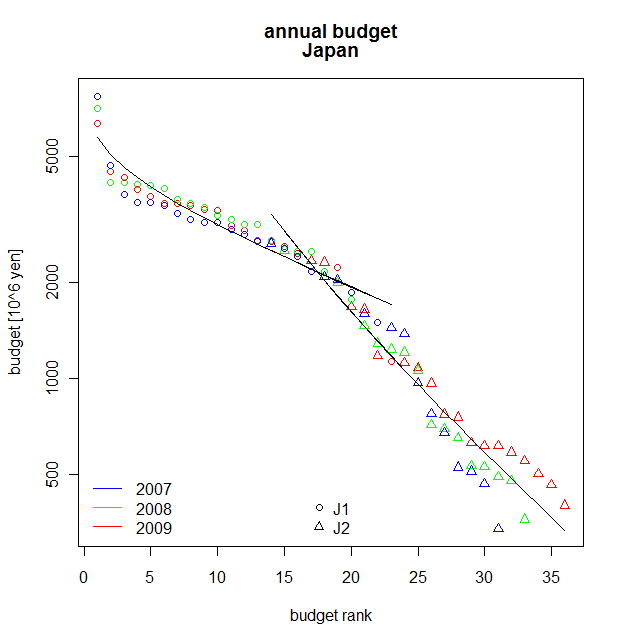
\includegraphics[width=.96\textwidth]{fig/japan-budget.png}
		\end{center}
		\caption{テスト}\label{fig:テスト}
	\end{figure} %}
%s3:Fock空間}
\subsubsection{非可換な係数}\label{s3:非可換な係数} %{
	可換上のBrzozowski代数を非可換上のBrzozowskiに拡張する。
	$V$を可換とは限らない環、$\Z V$を$V$の中心とする。
	$V\Eta(A):=V\otimes_{\Z V}(\Z V)\Eta(A)$と書き、$\otimes_{\Z V}$を省略して
	次のように書く。
	\begin{equation*}\begin{split}
		vx := v\otimes_{\Z V}x =: xv \\
		vx^\flat := v\otimes_{\Z V}x^\flat =: x^\flat v 
	\end{split}
		\quad\text{for all } v\in V,\; x\in(\Z V)\Eta(A)
	\end{equation*}
	また、テンソル積$V\Eta(A)\otimes_{\Z V}(\Z V)\Eta(A)$を多用するが、
	$V\Eta(A)\otimes\Eta(A):=V\Eta(A)\otimes_{\Z V}(\Z V)\Eta(A)$と略記する。
%s3:非可換な係数}
%s1:Brzozowski代数}
\section{Dyck単語の分割}\label{s1:Dyck単語の分割} %{
	この節では次の便宜を用いることにする。
	\begin{itemize}\setlength{\itemsep}{-1mm} %{
		\item Brzozowski代数 \\
		\item 係数の環 \\
		この節では、$V$を環、$\Z V$を$V$の中心として、
		テンソル積$x\otimes_{\Z C}y$を単に$x\otimes y$と省略する。
		\item Brzozowski代数の標準基底系 \\
		$V\Eta_*$の標準基底系を
		$\E_\pm\Eta_*:=\set{\eta_{\pm},\eta_{\pm2},\dots}$と書き、
		$\E\Eta_*:=\E_+\Eta_*$と略記する。
		\item 余積 \\
		$m_0:V\Eta_*\otimes(\Z C)\Eta_*\to V\Eta_*$を$V$-線形な文字列の連結
		とする。線形射$\Delta_0:V\Eta_*\to V\Eta_*\otimes(\Z V)\Eta_*$を
		$m_0$との交換関係によって定義する。
		\begin{equation*}\begin{split}
			xm_0 = m_0(\Delta_0x) \quad\text{for all } x\in V\Eta_*
		\end{split}\end{equation*}
		$\Eta_*$の標準基底系に対しては次のようになる。
		\begin{equation*}\begin{split}
			\Delta_0\eta_i = \eta_i\otimes1 + I_0\otimes\eta_i
			,\quad \Delta_0\eta_{-i} = \eta_{-i}\otimes1
			\quad\text{for all } i\in\sizen_+
		\end{split}\end{equation*}
		ここで、$I_0:=\ket{1}\bra{1}$と定義する。
		$\Delta_0$には左単位射がないので、余積にはならないが、
		代数射$V\Eta_*\to V\Eta_*\otimes(\Z V)\Eta_*$になっているので、
		Hopf代数の多くの性質を持つ。
	\end{itemize} %}

	\begin{todo}[リファクタリング]\label{todo:リファクタリング} %{
		以下には間違っているところがある。間違いを修正するついでにストーリーを
		整理する。
		\begin{itemize}\setlength{\itemsep}{-1mm} %{
			\item 間違い \\
			$\bra{w}\eta_K=\bra{\eta_K}\otimes\bra{w}
			\neq\bra{w}\otimes\bra{\eta_K}=\bra{\eta_K}w$
			%
			\item 部分真空期待値 \\
			任意の$n\in\sizen_+$に対して線形射$\J_n:V\Eta_*\to V\Eta_*$を
			次のように定義する。
			\begin{equation*}\begin{split}
				\eta_{\pm i}\J_n = \J_n\eta_{\pm i}
				\quad\text{for all } i\neq n\in\sizen_+,\quad
				\eta_n\J_n = 0 = \J_n\eta_{-n}
			\end{split}\end{equation*}
			文字集合$\E\Eta_*$から文字$\eta_n$を除いた集合を$\E\Eta_{-n}$と書くと、
			$\J_n$は形式的には$\sum_{w\in(\E\Eta_{-n})^*}\ket{w}\bra{w}$
			と書くことができる。本質的にはDiracのデルタ関数なので、存在するか
			どうかは微妙だと思う。
			%
			\item 余積の計算 \\
			$\xi_1,\dots,\xi_n\in\plr{\Z V}\E\Eta_*$として、$m_0$との交換関係
			を計算すると次のようになる。
			\begin{equation*}\begin{split}
				\xi_1\cdots\xi_n m_0 &= m_0\plr{\xi_1\cdots\xi_n \otimes1}
					+ \sum_{r=1}^n \xi_1\cdots\xi_{r-1} m_0
					\plr{I_0\xi_{r+1}\cdots\xi_n\otimes\xi_r} \\
				&= m_0\plr{\xi_1\cdots\xi_n \otimes1} + m_0 \sum_{r=1}^n 
					\plr{I_0\xi_{r+1}\cdots\xi_n\otimes\xi_1\cdots\xi_r} \\
			\end{split}\end{equation*}
		\end{itemize} %}
	\end{todo} %todo:リファクタリング}

	$V\Eta_n$への射影$I_n\in\End_V\plr{V\Eta_*}$を次のように定義すると、
	\begin{equation*}\begin{split}
		I_n := \sum_{w\in\Eta_{n+}^*}\ket{w^\flat}\bra{w}
	\end{split}\end{equation*}
	$I_n$は$\eta_{\pm1},\dots,\eta_{\pm n}$に対しては可換、
	$\eta_{\pm\plr{n+1}},\eta_{\pm\plr{n+2}},\dots$に対しては真空のように
	振る舞う。
	\begin{alignat*}{2}
		I_n\eta_{\pm i} &= \eta_{\pm i}I_n &\quad&\text{for all } i\in1..n \\
		I_n\eta_{-i} &= 0 = \eta_iI_n &\quad&\text{for all } n < i
	\end{alignat*}
	$I_n$を用いて射影$\braket{-}_n:V\Eta_*\to V\Eta_n$を次のように定義する。
	\begin{equation*}\begin{split}
		\braket{x}_n := I_nxI_n \quad\text{for all } x\in V\Eta_*
	\end{split}\end{equation*}

	$K\in\sizen$、$a,b,c\in V\Eta_K$とし、$\phi\in V\Eta_{K+1}$を次のように
	定義する。
	\begin{equation*}\begin{split}
		\phi := a + b\eta_{K+1} + \eta_{-\plr{K+1}}c
	\end{split}\end{equation*}
	Kleeneスターの射影$\braket{\phi^*}_K$を計算してみる。
	まず、次のようになるが、
	\begin{equation}\label{ea:Dyck単語の分割その一}\begin{split}
		I_K\phi^{n+2} &= a^{n+2}I_K 
			+ \sum_{r=0}^{n+1}a^rbI_K\eta_{K+1}\phi^{n+1-r} \\
	\end{split}\end{equation}
	$I_K^{1,2}$を次のように定義すると、
	\begin{equation*}\begin{split}
		I_K^{1,2} := \sum_{w\in\Eta_n^*}\ket{w^\flat}\bra{w}\otimes\bra{1}
	\end{split}\end{equation*}
	二項目の和の中は次のように書くことができる。
	\begin{equation*}\begin{split}
		I_K\eta_{K+1}\phi^{n+1-r}
		= I_K^{1,2} \plr{\id\otimes\eta_{K+1}}m_0^\flat\phi^{n+1-r}
	\end{split}\end{equation*}
	$\phi$と$m_0^\flat$の交換関係は次の形になるが、
	\begin{equation}\label{ea:Dyck単語の分割その二}\begin{split}
		m_0^\flat\phi &= \plr{\Delta_0\phi}m_0^\flat \\
		\Delta_0\phi &= \phi\otimes\id + I_0c\otimes\eta_{-\plr{K+1}}
			+ \plr{\cdots}\otimes\plr{\text{operators in $\Eta_{-K}$}}
	\end{split}\end{equation}
	生成演算子$\Eta_{K-}$がテンソル積の二項目に現れる項は
	$I_K\plr{\id\otimes\eta_{K+1}}$に作用すると$0$になるから、			
	次の式が成り立つ。
	\begin{equation}\label{ea:Dyck単語の分割その三}\begin{split}
		I_K\eta_{K+1}\phi^{n+1-r}
		&= I_K^{1,2} \plr{\id\otimes\eta_{K+1}}m_0^\flat\phi^{n+1-r} \\
		&= I_K^{1,2} \plr{\phi^{n+1-r}\otimes\eta_{K+1}} m_0^\flat \\
		&\;+ \sum_{s=0}^n I_K^{1,2} 
			\plr{\phi^sI_0c\otimes\eta_{K+1}\eta_{-\plr{K+1}}}
			m_0^\flat\phi^{n-(r+s)} \\
		&= I_K\phi^{n+1-r}\eta_{K+1} + \sum_{s=0}^n\phi^sI_0c\phi^{n-(r+s)}
	\end{split}\end{equation}
	したがって、次の式が得られる。
	\begin{equation*}\begin{split}
		I_K\phi^{n+2} &= a^{n+2}I_K 
			+ \sum_{r=0}^{n+1} a^rbI_K\phi^{n+1-r}\eta_{K+1}
			+ \sum_{r+s+t=n} a^rbI_K\phi^sI_0c\phi^t
	\end{split}\end{equation*}
	また、次の式が成り立つが、
	\begin{equation*}\begin{split}
		\braket{\phi^{n+2}}_K = a^{n+2} 
			+ \sum_{r+s+t=n} \braket{a^rb\phi^s}_KI_0\braket{c\phi^t}_K
	\end{split}\end{equation*}
	次の式を使うと、
	\begin{equation*}\begin{split}
		\braket{\phi^{n+3}}_K &= a^{n+3} + a\sum_{r+s+t=n}
			\braket{a^rb\phi^s}_KI_0\braket{c\phi^t}_K
			+ \sum_{r+s=n+1} \braket{b\phi^s}_KI_0\braket{c\phi^t}_K \\
		&= a\braket{\phi^{n+2}}_K + \sum_{s+t=n+1}
			\braket{b\phi^s}_KI_0\braket{c\phi^t}_K
	\end{split}\end{equation*}
	次の式より、
	\begin{equation*}\begin{split}
		\braket{\phi^0}_K &= 1 \\ 
		\braket{\phi^1}_K &= a\braket{\phi^0}_K \\ 
		\braket{\phi^2}_K &= a\braket{\phi^1}_K
			+ \sum_{s+t=0} \braket{b\phi^s}_KI_0\braket{c\phi^t}_K \\
		\braket{\phi^3}_K &= a\braket{\phi^2}_K 
			+ \sum_{s+t=1} \braket{b\phi^s}_KI_0\braket{c\phi^t}_K \\
		\cdots \\
	\end{split}\end{equation*}
	任意の$n\in\sizen$に対して次の式が成り立つ。
	\begin{equation*}\begin{split}
		\sum_{i=0}^{n+2} \braket{\phi^i}_K &= 1 
			+ \sum_{i=0}^{n+1} a\braket{\phi^i}_K 
			+ \sum_{s+t=n} \braket{b\phi^s}_KI_0\braket{c\phi^t}_K
	\end{split}\end{equation*}
	したがって、$t$を$V\Eta_*$の元と可換な不定元として、次の式が成り立つ。
	\begin{equation*}\begin{split}
		\Braket{\plr{t\phi}^*}_K = 1 + t\Braket{a\plr{t\phi}^*}_K 
			+ t^2\Braket{b\plr{t\phi}^*}_KI_0\Braket{c\plr{t\phi}^*}_K 
			\quad\text{up to } t^\infty
	\end{split}\end{equation*}
	この式は$t$の有限べきについて成り立つだけで、収束性
	$\braket{\phi^*}_K\in V\Eta_K$は保証していない。
	以上のことを命題の形でまとめておく。

	\begin{proposition}[Dyck単語の分割]\label{prop:Dyck単語の分割} %{
		$V$を環とする。$K\in\sizen$、$a,b,c\in V\Eta_K$として、
		$\phi\in V\Eta_{K+1}$を次のように定義すると、
		\begin{equation*}\begin{split}
			\phi := a + b\eta_{K+1} + \eta_{-\plr{K+1}}c
		\end{split}\end{equation*}
		形式級数$\braket{\plr{t\phi}^*}_K\in V\Eta_K[[t]]$について、次の式が
		成り立つ。
		\begin{alignat*}{2}
			\Braket{\plr{t\phi}^*}_K &= 1 + t\Braket{a\plr{t\phi}^*}_K 
				+ t^2\Braket{b\plr{t\phi}^*}_KI_0\Braket{c\plr{t\phi}^*}_K
				&\quad\text{up to } t^\infty \\
			&= \ggplr{ta + t^2b\Braket{\plr{t\phi}^*}_KI_0c}^* 
				&\quad\text{up to } t^\infty
		\end{alignat*}
		この式は$t$の有限べきについて成り立つだけで、
		収束性$\braket{\phi^*}_K\in V\Eta_K$は保証していない\footnote{
			無限和や無限積を含む場合は、有限和や有限積の場合に成り立つ事柄が
			そのまま成り立たないことが多い。代数的Chomsky-Schutzenberの定理
			\ref{s1:代数的Chomsky-Schutzenbergerの定理}を参照すること。
		}。
	\end{proposition} %prop:Dyck単語の分割}

	この命題から、$V[[t]]$に対する次の式が導かれる。
	\begin{equation*}\begin{split}
		\phi := a + b\eta_1 + \eta_{-1}c 
		\xRightarrow{x := \Braket{\plr{t\phi}^*}} x = 1 + tax + t^2bxcx
		\quad\text{for all } a,b,c\in V
	\end{split}\end{equation*}
	この式を$x=1+\plr{f|x}x$という形の文法に拡張することを考える。

	まず、二次式の範囲で考えてみる。$a,b_1,\dots,b_N,c_1,\dots,c_N\in V\Eta_K$
	として、$\phi\in V\Eta_{K+N}$を次のように定義する。
	\begin{equation*}\begin{split}
		\phi := a + \phi_+ + \phi_-
		,\quad \phi_+ := \sum_{i=1}^N b_i\eta_{K+i}
		,\quad \phi_- := \sum_{i=1}^N \eta_{-(K+i)}c_i
	\end{split}\end{equation*}
	式\eqref{ea:Dyck単語の分割その二}と同様に、次の式が成り立つから、
	\begin{equation*}\begin{split}
		m_0^\flat\phi &= \plr{\Delta_0\phi}m_0^\flat \\
		\Delta_0\phi &= \phi\otimes\id 
			+ \sum_{i=1}^N I_0c\otimes\eta_{-\plr{K+i}}
			+ \plr{\cdots}\otimes\plr{\text{operators in $\Eta_{-K}$}}
	\end{split}\end{equation*}
	任意の$n\in\sizen$で次の式が成り立ち、
	\begin{equation*}\begin{split}
		I_K\phi^{n+2} &= a^{n+2} + \sum_{r=0}^{n+1} a^rI_K\phi_+\phi^{n+1-r} \\
		&= a^{n+2} + \sum_{r=0}^{n+1} a^rI_K\phi^{n+1-r}\phi_+
			+ \sum_{r+s=n}\sum_{i=1}^N a^r\Braket{b_i\phi^s}I_0c_i\phi^{n-(r+s)}
	\end{split}\end{equation*}
	次の式が成り立つ。
	\begin{alignat*}{2}
		\Braket{\plr{t\phi}^*}_K &= 1 + ta\Braket{\plr{t\phi}^*}_K 
			+ t^2\sum_{i=1}^N\Braket{b_i\plr{t\phi}^*}_K
			I_0\Braket{c_i\plr{t\phi}^*}_K &\quad\text{up to }t^\infty \\
		&= \ggplr{ta + t^2\sum_{i=1}^N b_i\Braket{\plr{t\phi}^*}_KI_0c_i}^* 
			&\quad\text{up to } t^\infty
	\end{alignat*}
	以上のことを命題の形でまとめておく。

	\begin{proposition}[Dyck単語の分割その二]\label{prop:Dyck単語の分割その二} %{
		$V$を環とする。$K,N\in\sizen$、
		$a,b_1,\dots,b_N,c_1,\dots,c_N\in V\Eta_K$として、
		$\phi\in V\Eta_{K+N}$を次のように定義すると、
		\begin{equation*}\begin{split}
			\phi := a + \sum_{i=1}^N \plr{b_i\eta_{K+i} + \eta_{-(K+i)}c_i}
		\end{split}\end{equation*}
		次の式が成り立つ。
		\begin{alignat*}{2}
			\Braket{\plr{t\phi}^*}_K &= 1 + ta\Braket{\plr{t\phi}^*}_K 
				+ t^2\sum_{i=1}^N\Braket{b_i\plr{t\phi}^*}_K
				I_0\Braket{c_i\plr{t\phi}^*}_K &\quad\text{up to }t^\infty \\
			&= \ggplr{ta + t^2\sum_{i=1}^N b_i\Braket{\plr{t\phi}^*}_KI_0c_i}^* 
				&\quad\text{up to } t^\infty
		\end{alignat*}
	\end{proposition} %prop:Dyck単語の分割その二}

	単項式のべきについては次の命題が成り立つ。

	\begin{proposition}[Dyck単語の分割その三]\label{prop:Dyck単語の分割その三} %{
		$V$を環とする。$K,N\in\sizen$、$a,b_1,\dots,b_{N+2}\in V\Eta_K$として、
		$\phi\in V\Eta_{K+N+1}$を次のように定義すると、
		\begin{equation*}\begin{split}
			\phi := a + b_1\eta_{K+1} + \eta_{-(K+N+1)}b_{N+2} 
				+ \sum_{r=2}^{N+1} \eta_{-(K+r-1)}b_r\eta_{K+r}
		\end{split}\end{equation*}
		形式級数$\braket{\plr{t\phi}^*}_K\in V\Eta_K[[t]]$について、次の式が
		成り立つ。
		\begin{alignat*}{2}
			\Braket{\plr{t\phi}^*}_K &= 1 + t\Braket{A}_K
				+ t^{N+2}\Braket{B_1}_KI_0\Braket{B_2}\cdots\Braket{B_{N+1}}
				I_0\Braket{B_{N+2}}_K &\quad\text{up to } t^\infty \\
			&= \ggplr{ta 
				+ t^{N+2}\Braket{B_1}_KI_0\Braket{B_2}\cdots\Braket{B_{N+1}}
				I_0b_{N+2}}^* &\quad\text{up to } t^\infty
		\end{alignat*}
		ここで、$A$と$B_i$は次のように定義した。
		\begin{equation*}\begin{split}
			A := a\plr{t\phi}^*,\quad B_1 := b_1\plr{t\phi}^*,\dots,\quad 
			B_{N+2} := b_{N+2}\plr{t\phi}^*
		\end{split}\end{equation*}
		$B_1,\dots,B_{N+1}$に対しては部分真空期待値ではなく、
		完全な真空期待値をとっていることに注意する。
	\end{proposition} %prop:Dyck単語の分割その三}
	\begin{proof} %{
		命題の$N$の帰納法によって証明する。$N=0$のとき命題が成り立つことは
		Dyck単語の分割\ref{prop:Dyck単語の分割}からわかる。
		ある$N\in\sizen$で命題が成り立つと仮定し、$\phi_{N+3}\in V\Eta_{K+N+3}$
		を次のように定義する。
		\begin{equation*}\begin{split}
			\phi_{N+3} := a + b_1\eta_{K+1} + \eta_{-(K+N+2)}b_{N+3}
				+ \sum_{r=2}^{N+2} \eta_{-(K+r-1)}b_r\eta_{K+r}
		\end{split}\end{equation*}
		Dyck単語の分割\ref{prop:Dyck単語の分割}によって、$\eta_{\pm(K+N+3)}$を
		積分してしまうと、次の式が成り立つ。
		\begin{equation*}\begin{split}
			\Braket{\plr{t\phi_{N+3}}^*}_{K+N+2} = \plr{t\phi_{N+2}}^*
		\end{split}\end{equation*}
		ここで、$\phi_{N+2}\in V\Eta_{K+N+2}$は次のように定義した。
		\begin{equation*}\begin{split}
			\phi_{N+2} &:= a + b_1\eta_{K+1} + t\eta_{-(K+N+1)}c 
				+ \sum_{r=2}^{N+1} \eta_{-(K+r-1)}b_r\eta_{K+r} \\
			c &:= b_{N+2}\plr{t\phi_{N+2}}^*I_0 b_{N+3}\plr{t\phi_{N+2}}^*
		\end{split}\end{equation*}
		$\phi_{N+2}$は次の性質を持つことに注意して、
		\begin{equation*}\begin{split}
			\Braket{f\plr{t\phi_{N+2}}^*g}_K = \Braket{f\plr{t\phi_{N+3}}^*g}_K
			\quad\text{for all } f,g\in V\Eta_K
		\end{split}\end{equation*}
		$\phi_{N+2}$に対して帰納法の仮定を適用すると、次の式が得られるが、
		\begin{equation*}\begin{split}
			\Braket{\plr{t\phi_{N+2}}^*}_K
			= 1 + t\Braket{A}_K + t^{N+3}\Braket{B_1}_KI_0
				\Braket{B_2}\cdots\Braket{B_{N+1}}I_0
				\Braket{c\plr{t\phi_{N+2}}^*}_K \\
		\end{split}\end{equation*}
		次の式から、
		\begin{equation*}\begin{split}
			I_0\Braket{c\plr{t\phi_{N+2}}^*}_K = I_0\Braket{b_{N+2}
				\plr{t\phi_{N+2}}^*} I_0\Braket{b_{N+3}\plr{t\phi_{N+2}^*}}_K
			= I_0\Braket{B_{N+2}}I_0\Braket{B_{N+3}}_K
		\end{split}\end{equation*}
		次の式が成り立つことがわかる。
		\begin{equation*}\begin{split}
			\Braket{\plr{t\psi}^*}_K = 1 + t\Braket{A}_K 
				+ t^{N+3}\Braket{B_1}_KI_0\Braket{B_2}\cdots\Braket{B_{N+2}}
				I_0\Braket{B_{N+3}}_K
		\end{split}\end{equation*}
		したがって、
		$\Braket{\plr{t\phi_{N+3}}^*}_K=\Braket{\plr{t\phi_{N+2}}^*}_K$だから、
		$N+1$でも命題が成り立つことがわかる。
	\end{proof} %}

	この命題の$\phi$は次のベクトル$H_0,\; H_\pm$と巡回的な行列$B$を用いて、
	\begin{equation*}\begin{split}
		H_0 := \begin{pmatrix}
			1 \\ 0 \\ 0 \\ \vdots \\ 0 \\ 0
		\end{pmatrix},\quad H_\pm := \begin{pmatrix}
			0 \\ \eta_{\pm(K+1)} \\ \eta_{\pm(K+2)} 
			\\ \vdots \\ \eta_{\pm(K+N)} \\ \eta_{\pm(K+N+1)}
		\end{pmatrix},\quad B := \begin{pmatrix}
			0 & b_1 & 0 & 0 & \cdots & 0 \\
			0 & 0 & b_2 & 0 & \cdots & 0 \\
			0 & 0 & 0 & b_3 & \cdots & 0 \\
			\vdots & \vdots & \vdots & \vdots & \ddots & 0 \\
			0 & 0 & 0 & 0 & \cdots & b_{N+1} \\
			b_{N+2} & 0 & 0 & 0 & \cdots & 0 \\
		\end{pmatrix}
	\end{split}\end{equation*}
	次のように書くことができる。
	\begin{equation*}\begin{split}
		\phi = a + \plr{H_0 + H_-}^\tran B \plr{H_0 + H_+}
	\end{split}\end{equation*}
	メモ\ref{note:Dyck単語の分割その三}を使いつつ、
	行列の形で$\Braket{\phi^*}_K$を計算してみる。まず、Kleeneスターの摂動から
	次の式が成り立つが、
	\begin{equation*}\begin{split}
		\Braket{\phi^*}_K = 1 + \plr{a + H_0^\tran BH_0}\Braket{\phi^*}_K
			+ H_0^\tran B\Braket{H_+\phi^*}_K
	\end{split}\end{equation*}
	計算\eqref{eq:真空期待値の一次微分の計算}から、次の式が成り立つことが
	わかる。
	\begin{equation*}\begin{split}
		\Braket{H_+\phi^*}_K
		= 1 + \plr{a + H_0^\tran BB_\phi^*H_0}\Braket{\phi^*}_K
	\end{split}\end{equation*}
	ここで、$B_\phi\in(V\Eta_K)^{N+2}$は次のように定義する。
	\begin{equation*}\begin{split}
		B_\phi := \Braket{\phi^*}_KI_0\plr{1 - H_0H_0^\tran}B
	\end{split}\end{equation*}
	ここまでの計算結果は$B$の形に依らない。
	行列$B$の具体的な形を用いると、計算\eqref{eq:Bの具体形を用いた計算}から、
	命題の式が得られる。
	\begin{equation*}\begin{split}
		\Braket{\phi^*}_K
		= 1 + \plr{a + H_0^\tran BB_\phi^{N+1}H_0}\Braket{\phi^*}_K
	\end{split}\end{equation*}
	\begin{note}[計算メモ]\label{note:Dyck単語の分割その三} %{
		\begin{itemize}\setlength{\itemsep}{-1mm} %{
			\item $m_0^\flat\phi=\plr{\Delta_0\phi}m_0$とすると、次の式が
			成り立つ。
			\begin{equation*}\begin{split}
				\Delta_0\phi = \phi\otimes\id 
					+ I_0{\contraction{}{B(H_0 + H_+)}{\otimes}{H_-^\tran}
						B(H_0 + H_+)\otimes H_-^\tran}
					+ \plr{\cdots}\otimes\plr{\text{operators in $\Eta_{-K}$}}
			\end{split}\end{equation*}
			ここで、$\contraction{}{X}{\otimes}{Y^\tran}X\otimes Y^\tran$は
			次のようにテンソル積を跨いだベクトルの内積を表す。
			\begin{equation*}\begin{split}
				\contraction{}{X}{\otimes}{Y^\tran}X\otimes Y^\tran 
				:= \sum_{i=1}^{N+1}X_i\otimes Y_i
				,\quad \contraction{}{X^\tran}{\otimes}{Y}X^\tran\otimes Y
				:= \sum_{i=1}^{N+1}X_i\otimes Y_i
			\end{split}\end{equation*}
			%
			\item $\Braket{H_+\phi^*}_K$の計算
			\begin{equation*}\begin{split}
				I_KH_+\phi^* & = I_K^{1,2}(\id\otimes H_+)m_0^\flat\phi^* \\
				& = I_K^{1,2}(\phi^*\otimes H_+)m_0^\flat
					+ I_K^{1,2}(\phi^*\otimes H_+)
					\plr{I_0{\contraction{}{B(H_0 + H_+)}{\otimes}{H_-^\tran}
							B(H_0 + H_+)\otimes H_-^\tran}}
					m_0^\flat\phi^* \\
				&= I_K\phi^*H_+ + I_K\phi^*I_0\plr{H_+H_-^\tran}B(H_0 + H_+)\phi^*
			\end{split}\end{equation*}
			より、縮約に対する次の式と、
			\begin{equation*}\begin{split}
				\plr{\contraction{}{X_1^\tran}{\otimes}{Y_1} X_1^\tran\otimes Y_1}
				\plr{\contraction{}{X_2}{\otimes}{Y_2^\tran} X_2\otimes Y_2^\tran}
				&= \sum_{i,j} \plr{X_{1i}X_{2j}}\otimes\plr{Y_{1i}Y_{2j}} \\
				&= \contraction{(}{X_1}{\otimes1)(1\otimes}{Y_1}
				\contraction{(X_1\otimes1)(1\otimes Y_1}{Y_2^\tran}{)(}{X_2}
				(X_1\otimes1)(1\otimes Y_1Y_2^\tran)(X_2\otimes1)
			\end{split}\end{equation*}
			$H_\pm$に対する次の式を使って、
			\begin{equation*}\begin{split}
				H_+H_-^\tran = 1 - H_0H_0^\tran\in\text{ matrix of center of }V
			\end{split}\end{equation*}
			次の式が得られる。
			\begin{equation}\label{eq:真空期待値の一次微分の計算}\begin{split}
				\Braket{H_+\phi^*}_K 
				&= \Braket{\phi^*}_KI_0\plr{H_+H_-^\tran}BH_0\Braket{\phi^*}_K
				+ \Braket{\phi^*}_KI_0\plr{H_+H_-^\tran}B\Braket{H_+\phi^*}_K \\
				&= \ggplr{\Braket{\phi^*}_KI_0\plr{H_+H_-^\tran}B}^+H_0\Braket{\phi^*}_K
			\end{split}\end{equation}
			%
			\item $H_0^\tran BB_\phi^*H_0$の計算
			\begin{equation}\label{eq:Bの具体形を用いた計算}\begin{split}
				H_0^\tran BB_\phi^*H_0 &= \begin{pmatrix}
					0 \\ b_1 \\ 0 \\ \vdots \\ 0 \\ 0
				\end{pmatrix}^\tran\plr{\Braket{\phi^*}_KI_0\begin{pmatrix}
					0 & 0 & 0 & 0 & \cdots & 0 \\
					0 & 0 & b_2 & 0 & \cdots & 0 \\
					0 & 0 & 0 & b_3 & \cdots & 0 \\
					\vdots & \vdots & \vdots & \vdots & \ddots & 0 \\
					0 & 0 & 0 & 0 & \cdots & b_{N+1} \\
					b_{N+2} & 0 & 0 & 0 & \cdots & 0 \\
				\end{pmatrix}}^*\begin{pmatrix}
					1 \\ 0 \\ 0 \\ \vdots \\ 0 \\ 0
				\end{pmatrix} \\
				&= H_0^\tran BB_\phi^{N+1}H_0
			\end{split}\end{equation}
			$\beta_i$を次のようにおくと、
			\begin{equation*}\begin{split}
				\beta_1:=b_1,\quad
				\beta_i:=b_1\Braket{\phi^*}_KI_0b_2\cdots\Braket{\phi^*}_KI_0b_i
			\end{split}\end{equation*}
			次のようになっていることから、前記の式が成り立つことがわかる。
			\begin{equation*}\begin{split}
				H_0^\tran BB_\phi^0 &= (0\; \beta_1\; 0\; 0\; \cdots\; 0) \\
				H_0^\tran BB_\phi^1 &= (0\; 0\; \beta_2\; 0\; \cdots\; 0) \\
				\vdots \\
				H_0^\tran BB_\phi^N &= (0\; 0\; 0\; 0\; 0\; \cdots\; \beta_{N+1}) \\
				H_0^\tran BB_\phi^{N+1} H_0 &= (b_{N+2}\; 0\; 0\; 0\; \cdots\; 0) \\
				H_0^\tran BB_\phi^{N+2} H_0 &= (0\; 0\; 0\; 0\; \cdots\; 0)
			\end{split}\end{equation*}
		\end{itemize} %}
	\end{note} %note:Dyck単語の分割その三}
\subsection{観察その一}\label{s2:観察その一} %{
	この節では多項式とその根について考える。

	環$V$を係数とする多項式を$V$-多項式と書く事にする。通常は、多項式の
	係数は変数変換で変わり得るので、係数を明示することはないが、この節では
	多項式を変形していくので、係数を明示することにする。
	また、環$V$、$t$を$V$と可換な不定元として、
	\begin{itemize}\setlength{\itemsep}{-1mm} %{
		\item $V[t]$を$V$を係数とする$t$の多項式全体のつくる集合、
		\item $V[[t]]$を$V$を係数とする$t$の形式級数全体のつくる集合、
		\item $V(t):=V[t,t^{-1}]$、
		\item $V((t)):=V[[t,t^{-1}]]$、
	\end{itemize} %}
	とする。また、通常は用いられることがない記号だが、見やすさを考えて
	次の記法を使うことにする。
	\begin{equation*}\begin{split}
		[V]_t:=V[t],\quad [[V]]_t:=V[[t]],\quad (V)_t:=V[t,t^{-1}]
		,\quad ((V))_t:=V[[t,t^{-1}]]
	\end{split}\end{equation*}

	$t$を変数として次の$[\sei]_t$-多項式とその根$x_\pm\in((\fukuso))_t$
	を考える。
	\begin{equation}\label{eq:元の多項式}\begin{split}
		x = 1 + tx^2,\quad x_\pm := \frac{1 \pm \sqrt{1 - 4t}}{2t}
	\end{split}\end{equation}
	この多項式を次のプッシュダウンオートマトンを構成する過程に添って変形
	してみる。
	\begin{equation*}\begin{array}{rcll}
		\xymatrix{
			*++[o][F=]{x} \ar@(dl,ul)^{tx^2}
		} &\xmapsto{\text{insert final state}}& \xymatrix{
			*++[o][F-]{x} \ar[r]^{1+tx^2} & *++[o][F=]{y}
		} \\
		&\xmapsto{\text{eliminate 1st $x$}}& \xymatrix{
			*++[o][F-]{x} \ar[r]^{1} \ar@(dl,ul)^{t\eta_1} 
			& *++[o][F=]{y} \ar@(ru,rd)^{\eta_{-1}x}
		} \\
		&\xmapsto{\text{eliminate 2nd $x$}}& \xymatrix{
			*++[o][F-]{x} \ar@<1ex>[r]^{1} \ar@(dl,ul)^{t\eta_1} 
			& *++[o][F=]{y} \ar@(ru,rd)^{\eta_{-2}} \ar@<1ex>[l]^{\eta_{-1}\eta_2}
		}
	\end{array}\end{equation*}

	元の多項式\eqref{eq:元の多項式}の左辺で、$x=X/Y$という有理変換をして、
	次のように書き換える。
	\begin{equation*}\begin{split}
		X = xY ,\quad X = Y + tx^2Y
	\end{split}\end{equation*}
	この式は、任意の$g\neq0\in((\fukuso))_t$に対して
	$(X,Y)\mapsto\plr{gX,gY}$という変換で不変になっている。
	したがって、ある$y\neq0\in((\fukuso))_t$を用いて、$Y=y$としてゲージ固定
	すると、次の$((\fukuso))_t$-連立多項式が得られる。
	\begin{equation*}\begin{split}
		X = xY ,\quad X = Y + tx^2Y ,\quad Y = y
	\end{split}\end{equation*}
	\begin{equation*}\begin{split}
		\pvec{X}{Y} = \pvec{0}{y} + \begin{pmatrix}
			0 & 1 + tx^2 \\ 0 & 0
		\end{pmatrix}\pvec{X}{Y},\quad X = xY
	\end{split}\end{equation*}

	次の二つの$((\fukuso))_t$-連立多項式を考えると、
	それぞれの解$X^{(0\pm)}\in((\fukuso))_t^2$は唯一つ定まる
	\footnote{
		この代数式の書き換えはCole-Hopf変換に似ている。
		ポテンシャルが$x_\pm$、波動関数が$X^{(0\pm)}$に対応する。
	}。
	\begin{equation}\label{eq:多項式の線形化その零}\begin{split}
		X^{(0\pm)} = \pvec{0}{1} + \begin{pmatrix}
			0 & 1 + tx_\pm^2 \\ 0 & 0
		\end{pmatrix} X^{(0\pm)}
		\implies X^{(0\pm)} = \pvec{x_\pm}{1}
	\end{split}\end{equation}
	そして、この連立多項式を書き換えた次の二つの$[\fukuso]_t$-連立多項式も、
	それぞれの解$\what{X}^{(0\pm)}\in((\fukuso))_t^2$は唯一つ定まる。
	\begin{equation}\label{eq:多項式の線形化その零改}\begin{split}
		\what{X}^{(0\pm)} = \pvec{0}{1} + \begin{pmatrix}
			0 & 1 + t\what{X}^{(0\pm)}_1x_\pm \\ 0 & 0
		\end{pmatrix} \what{X}^{(0\pm)}
		\implies \what{X}^{(0\pm)} = \pvec{x_\pm}{1}
	\end{split}\end{equation}

	\begin{todo}[妄想あるいは]\label{todo:妄想あるいは} %{
		多項式の書き換え、\eqref{eq:多項式の線形化その零}
		から\eqref{eq:多項式の線形化その零改}、が本質的な気がしてきた。
		$x_\pm=1+tx_\pm^2$というのがゲージ変換に見えてきた。
	\end{todo} %todo:妄想あるいは}

	次の二つの$((\fukuso\Eta_1))_t$-連立多項式を考える。
	\begin{equation}\label{eq:多項式の線形化その一}\begin{split}
		X^{(1\pm)} = \pvec{0}{1} + T_{1\pm}X^{(1\pm)} 
		\quad\text{where } T_{1\pm} := \begin{pmatrix}
			t\eta_1 & 1 \\ 0 & \eta_{-1}x_\pm
		\end{pmatrix}
	\end{split}\end{equation}
	命題\ref{prop:Dyck経路の分割}から次の式が成り立ち、
	\begin{equation*}\begin{split}
		\braket{T_{1\pm}^*} = 1 + \begin{pmatrix}
			0 & 1 \\ 0 & 0
		\end{pmatrix}\braket{T_{1\pm}^*} + \begin{pmatrix}
			t & 0 \\ 0 & 0
		\end{pmatrix}\braket{T_{1\pm}^*}\begin{pmatrix}
			0 & 0 \\ 0 & x_\pm
		\end{pmatrix}\braket{T_{1\pm}^*}
	\end{split}\end{equation*}
	真空期待値は$((\fukuso))_t$-連立多項式\eqref{eq:多項式の線形化その零改}
	を再現する。
	\begin{equation*}\begin{split}
		\braket{X^{(1\pm)}} = \pvec{0}{1} + \begin{pmatrix}
			0 & 1 + t\braket{X^{(1\pm)}_1}x_\pm \\ 0 & 0
		\end{pmatrix} \braket{X^{(1\pm)}}
	\end{split}\end{equation*}
	ただし、$((\fukuso))_t$-連立多項式\eqref{eq:多項式の線形化その零改}の場合
	と異なり、遷移行列$T_{1\pm}$に$0$でない対角成分があるために、
	$\braket{T_{1\pm}^*}$が収束しない可能性がある。実際に$\braket{T_{1\pm}^*}$
	を計算すると次のようになり、
	\begin{equation*}\begin{split}
		\braket{T_{1\pm}^*} = 1 + \begin{pmatrix}
			0 & \plr{tx_\pm}^* \\ 0 & 0
		\end{pmatrix} \implies \braket{X^{(1\pm)}} = \pvec{\plr{tx_\pm}^*}{1}
	\end{split}\end{equation*}
	$\braket{T_{1\pm}^*}$が収束するためには、次の条件が必要なことがわかる。
	\begin{equation*}\begin{split}
		\plr{tx_\pm}^*\in\fukuso((t))
		\iff |tx_\pm| < 1
		\iff |1\pm\sqrt{1-4t}| < 2
	\end{split}\end{equation*}
	この条件は次の式を反映したものだから、
	\begin{equation*}\begin{split}
		x = 1 + tx^2 \iff x = \frac{1}{1 - tx}
		\implies x = \plr{tx}^* \quad\text{iff}\quad |tx| < 1
	\end{split}\end{equation*}
	この条件が満たされるときに限り、$x_\pm=\plr{tx_\pm}^*$となる。
	つまり、
	\begin{itemize}\setlength{\itemsep}{-1mm} %{
		\item 真空期待値$\braket{X^{(1\pm)}}$が収束するならば、
		$\braket{X^{(1\pm)}}=(x_\pm,\; 1)^\tran$となる
	\end{itemize} %}
	ということが言える。式で書くと次のようになる。
	\begin{equation}\label{eq:多項式の収束条件その一}\begin{split}
		\braket{X^{(1\pm)}}\in((\fukuso))_t
		\implies \braket{X^{(1\pm)}} = \pvec{x_\pm}{1}
	\end{split}\end{equation}
%	そして、$\braket{X^{(1\pm)}}\in((\fukuso))_t$となるときは、
%	$((\fukuso\Eta_1))_t$-連立多項式\eqref{eq:多項式の線形化その一}を
%	次のように、$[\fukuso\Eta_1]_t$-連立多項式に書き換えることができる。
%	\begin{equation}\label{eq:多項式の線形化その一改}\begin{split}
%		\what{X}^{(1)} = \pvec{0}{1} + \what{T}_{1}\what{X}^{(1)}
%		\quad\text{where } \what{T}_{1} := \begin{pmatrix}
%			t\eta_1 & 1 \\ 0 & \eta_{-1}\braket{\what{X}^{(1)}_1}
%		\end{pmatrix}
%	\end{split}\end{equation}
%	この連立多項式には$x_\pm$が現れないので、$t$の多項式を係数とすることに
%	注意する。

	次の$[\fukuso\Eta_2]_t$-連立多項式を考える。
	\begin{equation}\label{eq:多項式の線形化その二}\begin{split}
		X^{(2)} = \pvec{0}{1} + T_{2}X^{(2)} 
		\quad\text{where } T_{2} := \begin{pmatrix}
			t\eta_1 & 1 \\ \eta_{-1}\eta_2 & \eta_{-2}
		\end{pmatrix}
	\end{split}\end{equation}
	命題\ref{prop:Dyck経路の分割}から、部分真空期待について次の式が成り立ち、
	\begin{equation*}\begin{split}
		\braket{T_{2}^*}_1 = 1 + \begin{pmatrix}
			t\eta_1 & 1 \\ 0 & 0
		\end{pmatrix}\braket{T_{2}^*}_1 + I_1\begin{pmatrix}
			0 & 0 \\ \eta_{-1} & 0
		\end{pmatrix}T_{2}^*I_0\begin{pmatrix}
			0 & 0 \\ 0 & 1
		\end{pmatrix}T_{2}^*I_1 
	\end{split}\end{equation*}
	$((\fukuso\Eta_1))_t$-連立多項式\eqref{eq:多項式の線形化その一}に似ている
	が異なる次の$[\fukuso\Eta_1]_t$-連立多項式が得られる。
	\begin{equation*}\begin{split}
		Y^{(1)} = \pvec{0}{1} + \begin{pmatrix}
			t\eta_1 & 1 \\ 0 & \eta_{-1}Y^{(1)}_1I_0
		\end{pmatrix} Y^{(1)}
		\quad\text{where } Y^{(1)} := \braket{X^{(2)}}_1
	\end{split}\end{equation*}

	\begin{todo}[多項式の係数を明示]\label{todo:多項式の係数を明示} %{
	\end{todo} %todo:多項式の係数を明示}

	\begin{todo}[以下は怪しい]\label{todo:以下は怪しい} %{
		結果は正しいが、議論はおかしい。
	\end{todo} %todo:以下は怪しい}

	この連立多項式と連立多項式\eqref{eq:多項式の線形化その一改}は異なるが、
	真空期待値をとると同じ連立多項式となる。
	\begin{equation*}\begin{split}
		\Braket{X^{(1)}} &= \pvec{0}{1} + \Braket{\begin{pmatrix}
			t\eta_1 & 1 \\ 0 & 0
		\end{pmatrix} X^{(1)}} \\
		\Braket{\braket{X^{(2)}}_1} &= \pvec{0}{1} + \Braket{\begin{pmatrix}
			t\eta_1 & 1 \\ 0 & 0
		\end{pmatrix} \braket{X^{(2)}}_1}
	\end{split}\end{equation*}

	\begin{equation*}\begin{split}
		\braket{T_{2}^*} = 1 + \Braket{\begin{pmatrix}
			t\eta_1 & 1 \\ 0 & 0
		\end{pmatrix}T_{2}^*} + \Braket{\begin{pmatrix}
			0 & 0 \\ \eta_{-1} & 0
		\end{pmatrix}T_{2}^*}\Braket{\begin{pmatrix}
			0 & 0 \\ 0 & 1
		\end{pmatrix}T_{2}^*}
	\end{split}\end{equation*}

	部分真空期待値として$\fukuso\Eta_1((t))$上の連立代数式
	\eqref{eq:多項式の線形化その一改}が再現される。
	\begin{equation*}\begin{split}
		\braket{X^{(2)}}_1 = \pvec{0}{1} + \begin{pmatrix}
			t\eta_1 & 1 \\ 0 & \eta_{-1}\braket{X^{(2)}_1}_1
		\end{pmatrix} \braket{X^{(2)}}_1
	\end{split}\end{equation*}
	$\braket{X^{(2)}}$を具体的に計算してみたいところだが、$T_2^*$は次の
	ようになり、
	\begin{equation*}\begin{split}
		T_2^* = U_1\plr{1 + U_2}U_3^* \quad\text{where }
		U_1 = \begin{pmatrix}
			\plr{t\eta_1}^* & 0 \\ 0 & \eta_{-2}^*
		\end{pmatrix},\quad U_2 = \begin{pmatrix}
			0 & \eta_{-2}^* \\ \eta_{-1}\eta_2\plr{t\eta_1}^* & 0
		\end{pmatrix} \\
		U_3 = \begin{pmatrix}
			\eta_{-2}^*\eta_{-1}\eta_2\plr{t\eta_1}^* & 0 \\
			0 & \eta_{-1}\plr{\eta_2\plr{t\eta_1}^* + \eta_{-2}^*} \\
		\end{pmatrix}
	\end{split}\end{equation*}
	収束性を議論できるところまで持っていくことが困難である。
	したがって、$\braket{T_2^*}$の具体的な計算をせずにその収束性を考える。
	$T_2$は$t$の一次式だから、$\braket{T_2^*}$は$t$の形式級数となる。
	\begin{equation*}\begin{split}
		\braket{T_2^*}\in\fukuso[[t]]\subset\fukuso((t))
		\implies \braket{X^{(2)}}\in\fukuso[[t]]
	\end{split}\end{equation*}
	したがって、真空期待値が収束するための条件は、$\fukuso\Eta_1((t))$上の
	連立多項式の場合\eqref{eq:多項式の収束条件その一}より更に厳しく、
	次のようになる。
	\begin{equation*}\begin{split}
		\braket{X^{(2)}}\in\fukuso[[t]]
		\implies \braket{X^{(2)}} = \pvec{x_-}{1}
	\end{split}\end{equation*}
	$x_+$は$t=0$近傍で正則でないので、この連立多項式
	\eqref{eq:多項式の線形化その二}の根に含まれない。

	\begin{todo}[摂動展開の基点]\label{todo:摂動展開の基点} %{
		ここでの議論は$t=0$近傍で摂動展開しているが、任意の複素数$t_0\in\fukuso$
		を基点に摂動展開できるはずである。
	\end{todo} %todo:摂動展開の基点}
%s2:観察その一}
\subsection{観察その二}\label{s2:観察その二} %{
	前節の$\fukuso\Eta_2((t))$上の連立代数式\eqref{eq:多項式の線形化その二}
	は次のもので、
	\begin{equation*}\begin{split}
		X^{(2)} = \pvec{0}{1} + T_{2}X^{(2)} 
		\quad\text{where } T_{2} := \begin{pmatrix}
			t\eta_1 & 1 \\ \eta_{-1}\eta_2 & \eta_{-2}
		\end{pmatrix}
	\end{split}\end{equation*}
	部分真空期待は次の式を満たす。
	\begin{equation*}\begin{split}
		\braket{T_{2}^*}_1 = 1 + \begin{pmatrix}
			t\eta_1 & 1 \\ 0 & 0
		\end{pmatrix}\braket{T_{2}^*}_1 + I_1\begin{pmatrix}
			0 & 0 \\ \eta_{-1} & 0
		\end{pmatrix}T_{2}^*\ket{1}\bra{1}\begin{pmatrix}
			0 & 0 \\ 0 & 1
		\end{pmatrix}T_{2}^*I_1
	\end{split}\end{equation*}
	ここで、次の式が成り立つから、
	\begin{equation*}\begin{split}
		\begin{pmatrix}0 & 1\end{pmatrix}\bra{1}T_{2} = 0
	\end{split}\end{equation*}
	部分真空期待は次のようになる。
	\begin{equation*}\begin{split}
		\braket{T_{2}^*}_1 = 1 + \begin{pmatrix}
			t\eta_1 & 1 \\ 0 & 0
		\end{pmatrix}\braket{T_{2}^*}_1 + I_1\begin{pmatrix}
			0 & 0 \\ \eta_{-1} & 0
		\end{pmatrix}T_{2}^*\ket{1}\bra{1}\begin{pmatrix}
			0 & 0 \\ 0 & 1
		\end{pmatrix}I_1
	\end{split}\end{equation*}
%s2:観察その二}
\subsection{バックアップ}\label{s2:バックアップ} %{
	Dyck経路の分割\ref{eq:Dyck経路の分割}を行列に
	応用してみる。$V$を環、$K\in\sizen$をBrzozowski代数の階数、
	$D\in\sizen_+$を$V$上の自由加群の次元、
	\begin{itemize}\setlength{\itemsep}{-1mm} %{
		\item $X_0\in V^D$を初期値、
		\item $Y\in\plr{V\Eta_K}^D$をあるベクトル、
		\item $A,B\in\Mat\plr{V\Eta_K,D}$を行列
	\end{itemize} %}
	として、$X\in\plr{V\Eta_{K+1}}^{K+1}$を次の代数式の解とすると、
	\begin{equation*}\begin{split}
		X = X_0 + \plr{A + B\eta_{K+1} + \eta_{-\plr{K+1}}X_0Y^\tran}X
	\end{split}\end{equation*}
	Dyck経路の分割\ref{eq:Dyck経路の分割}により、
	次の$\plr{V\Eta_{K+1}}^{K}$の代数式が得られる。
	\begin{equation*}\begin{split}
		[X]_K = X_0 + A[X]_K + B[X]_K\ket{1}\bra{1}Y^\tran[X]_K
	\end{split}\end{equation*}
%s2:バックアップ}
%s1:Dyck経路の分割}
\section{木の成長とDyck経路の成長}\label{s1:木の成長とDyck経路の成長} %{
	Brzozowski代数によるDyck経路の成長$g:=b\eta\plr{\eta^\flat c}^*$を、
	$q=0$の平面二分木の成長に対応させてみる。

	一次、$\bra{1}\mapsto\bra{1}g$、は次のように、
	\begin{equation*}\begin{split}
		\sbt &\mapsto \smallxy{
			& \sbt \hen[dl] \\
			\sbt \\
		} +  \smallxy{
			& \sbt \hen[dl] \hen[dr] \\
			\sbt & & \sbt \\
		}
	\end{split}\end{equation*}
	二次、$\bra{1}g\mapsto\bra{1}g^2$、は次のように、
	\begin{equation*}\begin{split}
		\smallxy{
			& \sbt \hen[dl] \\
			\sbt \\
		} &\mapsto \smallxy{
			& & \sbt \hen[dl] \\
			& \sbt \hen[dl] \\
			\sbt \\
		} + \smallxy{
			& & \sbt \hen[dl] \\
			& \sbt \hen[dl] \hen[dr] \\
			\sbt & & \sbt \\
		} + \smallxy{
			& & \sbt \hen[dl] \hen[dr] \\
			& \sbt \hen[dl] \hen[dr] & & \sbt \\
			\sbt & & \sbt \\
		} \\
		\smallxy{
			& \sbt \hen[dl] \hen[dr] \\
			\sbt & & \sbt \\
		} &\mapsto \smallxy{
			& \sbt \hen[dl] \hen[dr] \\
			\sbt & & \sbt \hen[dl] \\
			& \sbt \\
		} + \smallxy{
			& \sbt \hen[dl] \hen[dr] \\
			\sbt & & \sbt \hen[dl] \hen[dr] \\
			& \sbt & & \sbt \\
		}
	\end{split}\end{equation*}
	三次、$\bra{1}g^2\mapsto\bra{1}g^3$、は次のようになる。
	\begin{equation*}\begin{array}{rcccccccc}
		\smallxy{
			& & \sbt \hen[dl] \\
			& \sbt \hen[dl] \\
			\sbt \\
		} &\mapsto& \smallxy{
			& & & \sbt \hen[dl] \\
			& & \sbt \hen[dl] \\
			& \sbt \hen[dl] \\
			\sbt \\
		} &+& \smallxy{
			& & & \sbt \hen[dl] \\
			& & \sbt \hen[dl] \\
			& \sbt \hen[dl] \hen[dr] \\
			\sbt & & \sbt \\
		} &+& \smallxy{
			& & & \sbt \hen[dl] \\
			& & \sbt \hen[dl] \hen[dr] \\
			& \sbt \hen[dl] \hen[dr] & & \sbt \\
			\sbt & & \sbt \\
		} &+& \smallxy{
			& & & \sbt \hen[dl] \hen[dr] \\
			& & \sbt \hen[dl] \hen[dr] & & \sbt \\
			& \sbt \hen[dl] \hen[dr] & & \sbt \\
			\sbt & & \sbt \\
		} \\
		\smallxy{
			& & \sbt \hen[dl] \\
			& \sbt \hen[dl] \hen[dr] \\
			\sbt & & \sbt \\
		} &\mapsto& \smallxy{
			& & \sbt \hen[dl] \\
			& \sbt \hen[dl] \hen[dr] \\
			\sbt & & \sbt \hen[dl] \\
			& \sbt
		} &+& \smallxy{
			& & \sbt \hen[dl] \\
			& \sbt \hen[dl] \hen[dr] \\
			\sbt & & \sbt \hen[dl] \hen[dr] \\
			& \sbt & & \sbt
		} &+& \smallxy{
			& & \sbt \hen[dl] \hen[dr] \\
			& \sbt \hen[dl] \hen[dr] & & \sbt \\
			\sbt & & \sbt \hen[dl] \hen[dr] \\
			& \sbt & & \sbt
		} \\
		\smallxy{
			& \sbt \hen[dl] \hen[dr] \\
			\sbt & & \sbt \hen[dl] \\
			& \sbt \\
		} &\mapsto& \smallxy{
			& \sbt \hen[dl] \hen[dr] \\
			\sbt & & \sbt \hen[dl] \\
			& \sbt \hen[dl] \\
			\sbt \\
		} &+& \smallxy{
			& \sbt \hen[dl] \hen[dr] \\
			\sbt & & \sbt \hen[dl] \\
			& \sbt \hen[dl] \hen[dr] \\
			\sbt & & \sbt \\
		} &+& \smallxy{
			& \sbt \hen[dl] \hen[dr] \\
			\sbt & & \sbt \hen[dl] \hen[dr] \\
			& \sbt \hen[dl] \hen[dr]  & & \sbt \\
			\sbt & & \sbt \\
		} \\
		\smallxy{
			& & \sbt \hen[dl] \hen[dr] \\
			& \sbt \hen[dl] \hen[dr] & & \sbt \\
			\sbt & & \sbt \\
		} &\mapsto& \smallxy{
			& & \sbt \hen[dl] \hen[dr] \\
			& \sbt \hen[dl] \hen[d] & & \sbt \hen[d] \\
			\sbt & \sbt & & \sbt \\
		} &+& \smallxy{
			& & \sbt \hen[dl] \hen[dr] \\
			& \sbt \hen[dl] \hen[d] & & \sbt \hen[d] \hen[dr] \\
			\sbt & \sbt & & \sbt & \sbt \\
		} \\
		\smallxy{
			& \sbt \hen[dl] \hen[dr] \\
			\sbt & & \sbt \hen[dl] \hen[dr] \\
			& \sbt & & \sbt \\
		} &\mapsto& \smallxy{
			& \sbt \hen[dl] \hen[dr] \\
			\sbt & & \sbt \hen[dl] \hen[dr] \\
			& \sbt & & \sbt \hen[dl] \\
			& & \sbt \\
		} &+& \smallxy{
			& \sbt \hen[dl] \hen[dr] \\
			\sbt & & \sbt \hen[dl] \hen[dr] \\
			& \sbt & & \sbt \hen[dl] \hen[dr] \\
			& & \sbt & & \sbt \\
		} \\
	\end{array}\end{equation*}
	成長$\bra{1}g^n\mapsto\bra{1}g^{n+1}$を平面二分木の言葉で書くと次のように
	なるだろう。
	\begin{itemize}\setlength{\itemsep}{-1mm} %{
		\item 行きがけ順で最後の葉$p$を見つける。
		\item $p$に左の子供を付け足す。
		\item 行きがけ順で$p$の後ろの頂点に右の子供を付け足す。
	\end{itemize} %}
	次のように対応する。
	\begin{equation*}\begin{array}{rcccccccc}
		\bra{1}(b\eta)(bc)b\eta(\eta^\flat c)^*
		&=& \bra{1}(b\eta)(bc)(b\eta) &+& \bra{1}(b\eta)(bc)(bc)
		&+& \bra{1}(b)(bc)(bc^2) \\
		\smallxy{
			& & \sbt \hen[dl] \\
			& \sbt \hen[dl] \hen[dr] \\
			\sbt & & \sbt \\
		} &\mapsto& \smallxy{
			& & \sbt \hen[dl] \\
			& \sbt \hen[dl] \hen[dr] \\
			\sbt & & \sbt \hen[dl] \\
			& \sbt
		} &+& \smallxy{
			& & \sbt \hen[dl] \\
			& \sbt \hen[dl] \hen[dr] \\
			\sbt & & \sbt \hen[dl] \hen[dr] \\
			& \sbt & & \sbt
		} &+& \smallxy{
			& & \sbt \hen[dl] \hen[dr] \\
			& \sbt \hen[dl] \hen[dr] & & \sbt \\
			\sbt & & \sbt \hen[dl] \hen[dr] \\
			& \sbt & & \sbt
		} \\
	\end{array}\end{equation*}
	この
%s1:木の成長とDyck経路の成長}
%
}\endgroup %}
